\documentclass[a4paper,11pt,twoside]{article}
\usepackage[absolute,overlay]{textpos}
\usepackage[english]{babel} %% needed for refs not to get a "~"

\usepackage{lscape}
\usepackage{array}
\usepackage{geometry}
\geometry{verbose,a4paper,tmargin=23mm,bmargin=26mm,lmargin=30mm,rmargin=30mm}

\usepackage{setspace}
\singlespacing

\usepackage{graphicx}

\usepackage[latin1]{inputenc}
\usepackage{times}
\usepackage[T1]{fontenc}

\setcounter{secnumdepth}{5} %% paragraphs in toc
\setcounter{tocdepth}{5}


\usepackage{datetime} %% but I think I am not using it


\usepackage{tikz}
\usetikzlibrary{arrows,shapes,positioning}

\tikzset{
  % Define standard arrow tip
  >=stealth',
  % Define style for boxes
  punkt/.style={
    rectangle,
    rounded corners,
    draw=black, %very thick,
    %maximum width=6em,
    %text width=6.5em,
    minimum height=2em,
    text centered},
  punkt2/.style={
    rectangle,
    rounded corners,
    draw=black, %very thick,
    text width=2.35cm,
    %text width=6.5em,
    minimum height=2em,
    inner sep = 2pt,
    text centered},
  punkt3/.style={
    rectangle,
%    rounded corners,
    draw=black, %very thick,
%    text width=1.cm,
    %text width=6.5em,
    minimum height=2em,
    inner sep = 3pt,
    text centered},
  punkk/.style={
    rectangle,
    rounded corners=3mm,
    draw=black, %very thick,
    %text width=6.5em,
    minimum height=2em,
    text centered},
  ell1/.style={
    %ellipse,
    %draw = black, very thick,
    text width=1.7cm,
    inner sep = 0pt,
    text centered},
  % Define arrow style
  pil/.style={
    ->,
    thick,
    shorten <=2pt,
    shorten >=2pt,}
}




\usepackage{verbatim}
\usepackage{amsmath}
\usepackage[hyphens]{url}
\usepackage[pdftex]{hyperref}
%\usepackage{cite}

\usepackage{url}
\usepackage{xcolor}
\definecolor{light-gray}{gray}{0.72}
\newcommand{\cyan}[1]{{\textcolor {cyan} {#1}}}
\newcommand{\blu}[1]{{\textcolor {blue} {#1}}}
\newcommand{\Burl}[1]{\blu{\url{#1}}}
\newcommand{\Curl}[1]{{\small \url{#1}}} %% you need to scape #

\newcommand{\lgray}[1]{{\textcolor {light-gray} {#1}}}
\newcommand{\red}[1]{{\textcolor {red} {#1}}}
\newcommand{\green}[1]{{\textcolor {green} {#1}}}
\newcommand{\mg}[1]{{\textcolor {magenta} {#1}}}
\newcommand{\og}[1]{{\textcolor {PineGreen} {#1}}}
%\newcommand{\code}[1]{\texttt{\slshape\footnotesize #1}}
%\newcommand{\code}[1]{\texttt{\slshape #1}}
\newcommand{\code}[1]{\texttt{#1}}
\newcommand{\opage}[1]{\texttt{[p.\ #1]}}
\newcommand{\myverb}[1]{{\footnotesize\texttt {\textbf{#1}}}}
\newcommand{\Rnl}{\ +\qquad\ }
\newcommand{\Emph}[1]{\emph{\mg{#1}}}

\providecommand{\tabularnewline}{\\}

%\usepackage{harvard}
\usepackage[authoryear, round, sort]{natbib}
\bibliographystyle{myagsm} %%bbs and chicago does not show URLs 
%%bbs and chicago does not show URLs 

% /texmf/bibtex/bst/myagsm.bst
% and then do texhash

%% Algorithm2e needs to come after natbib!!
\usepackage[boxed,vlined,linesnumbered]{algorithm2e}


%% \usepackage{enumitem} %% not clear I need it
\usepackage{enumerate}

%% an ugly hack, because I cannot get anything else to work

% \newlist{exsection}{enumerate}{10}
% \setlist[exsection]{label*=\thesection.\arabic*.}

% \newlist{exsubsection}{enumerate}{10}
% \setlist[exsubsection]{label*=\thesubsection.\arabic*.}

% \newlist{exsubsubsection}{enumerate}{10}
% \setlist[exsubsubsection]{label*=\thesubsubsection.\arabic*.}


% \DeclareMathOperator*{\argmax}{arg\,max}
% \underset{x}{\operatorname{argmax}}



\title{Classical algorithms in bioinformatics. Algorithms, probability,
  dynamic programming, HMMs. \\ \vspace*{25pt} \large  Class notes for BM-13, ``Bioinform�tica Avanzada y
Biolog�a de Sistemas'', 2014-2015.}

\author{Ram�n Diaz-Uriarte\\
              Dept. Bioqu�mica\\Universidad Aut�noma de Madrid \\ 
              \texttt{ramon.diaz@iib.uam.es} \\ 
              \Burl{http://ligarto.org/rdiaz} }


\date{\gitAuthorDate\ {\footnotesize (Release\gitRels: Rev:
    \gitAbbrevHash)}}


%\date{}

%\date{\ddmmyyyydate \today} %needs datetime package
% \date{\the\year-\the\month-\the\day}


\makeindex


\begin{document}

\maketitle
\vspace{-0.5cm}


\tableofcontents
\clearpage


\section{Pedagogical and scientific objectives of this module}
This module will introduce basic ideas about algorithms and probability,
and will then go into a certain amount of detail about sequence alignment,
dynamic programming, and hidden markov models. These are several of the
main objectives:

\begin{itemize}
\item Familiarize you with dynamic programming, a very common algorithm
  used in many different problems in bioinformatics (and elsewhere). As a
  side effect, familiarize you with algorithmic thinking (abstracting the
  unneeded details to get to the computational recipe).
\item In the process, get a better understanding of the sequence alignment
  problem, and what alignment scores are.
\item Review some probability ideas that will be used in several other
  places through the course and are fundamental for scientific inference.
\item Familiarize you with Hidden Markov Models, another widely used
  modeling tool. Have you play with HMMs as a way of both understanding
  HMMs and, more generally, seeing probabilistic models in practice, and
  yet another application of dynamic programming.
\item Be aware that successful computational approaches are based on
  rigorous, statistically sound methods. At the same time, that methods
  make assumptions that might, or might not, make sense for our problem.
\item Start reading papers from the primary bioinformatics/computational
  biology literature to get answers to our bioinformatics/computational
  needs. 
\end{itemize}




\section{Introduction to algorithms}


\subsection{What is an algorithm}

An algorithm is a sequence of instructions to solve a problem. Other
definitions refer to an algorithm as a recipe for carrying out a
computational task  \citep[preface to][]{Pevzner2011}. Given a
set of inputs, an algorithm will produce an output, following a clearly
specified, unambiguous, set of operations. Note, however, that the output
need not be deterministic.

Algorithms are often represented as pseudocode; pseudocode is not written
in any specific programming language, and avoids many of the details of
programming languages, but is much more precise than natural language.


Figure \ref{algo-examples} \citep[from p.\ 33 in][]{Jones} shows two
different algorithms to compute the $n$th Fibonacci number. The first is
recursive, while the second is iterative. You should be able to understand
what each is doing, and why we say one is recursive and the other
iterative. Other algorithms, of course, can be much more complicated.


 \begin{figure}[h!]
%   \begin{center}
     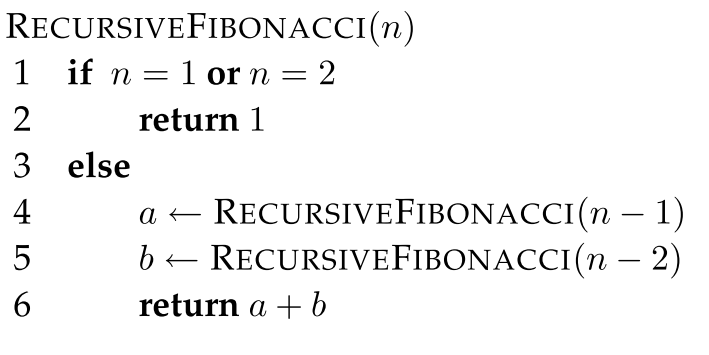
\includegraphics[width=8.1cm,keepaspectratio]{fibo-recurse.png}

\vspace*{8pt}


     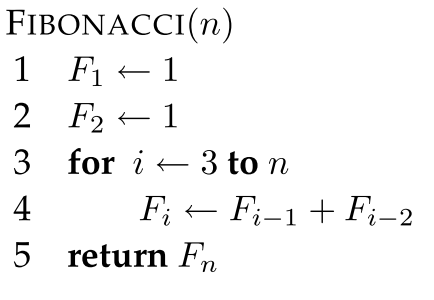
\includegraphics[width=5.1cm,keepaspectratio]{fibo-iterate.png}
%   \end{center}
\caption{\label{algo-examples} Two different algorithms for the Fibonacci
  numbers \citep[from p.\ 33 in][]{Jones}.
}
 \end{figure}



\subsection{Big-O notation}

We often care about how fast our algorithm will be. Timing it on a
specific machine might not be very helpful. It is often better to
understand the number of operations that have to be performed.  For
instance, suppose an algorithm that takes one list of numbers, of length
$n$, and does something to it. This algorithm might need, say, $3*n�$
operations. Then, this algorithm is said to be of order $n^2$, or
$O(n^2)$. In other words, the number of operations is proportional to the
square of the size of the input, or the time the algorithm needs grows
quadratically with the size of the input. More precisely, it really means
that the running time will grow no faster than the square of the size of
the input (or the running time is bounded from above by a function that
grows as $n^2$).

What happened to the ``3''? As $n$ grows larger, the constant ``3'' is not
very important. For instance, with large $n$, something that takes $3n�$
will run in a lot less time than something that takes $0.7n^3$. Of course,
when $n$ is small, the ``3'' could make a difference.


Other algorithms do things to different sets of numbers (as we will see
with sequence alignment); for instance, having as input one list of length
$n$ and another of length $m$. Then, maybe this algorithm will be of order
$O(nm)$, meaning that the number of operations are proportional to the
product of the sizes of the inputs. If $n$ and $m$ are of about the same
size, we often say the algorithm is of $O(n^2)$.

Some algorithms are $O(1)$, which is neat, since they run in constant
time, regardless of size of input. Nowadays, algorithm $O(n^2)$ are slow
but for many purposes acceptable. $O(n^3)$ algorithms, however, are only
useful for very small problems.

Some algorithms are $O(n^k)$ (e.g., $k = 2$), and these algorithms are of
polynomial complexity. Other algorithms are $O(k^n)$, for instance
$O(2^n)$, and these are called exponential ($n$ is in the exponent). An
algorithm of $O(2^n)$, for instance, will take twice as long with an input
of size $n + 1$ compared to an input of size $n$.

% (this is taken from Skiena's excellent text)

This is an ordering of some common dominance relationships between classes
of functions that you will find in the literature:

$n! \gg 2^n \gg n^3 \gg n^2 \gg n \log n \gg \log n \gg 1$

That ordering means that functions in the class of functions $f(\log n)$ dominate, or grow
faster, than functions in the class $f(1)$, or constant functions;
functions in the class of functions $f(n)$ grow faster than those in the
class $f(\log n)$, etc. 


We have mentioned number of operations, but similar concerns apply to
memory storage: how much memory an algorithm needs to run. Again, we
express this using the big-O notation.


Oh, and you should remember that, when thinking about a problem, we might
consider the average case, the worst case, and the best case. Therefore,
you might see expressions like \textit{worst-case complexity},
\textit{average-case complexity} and \textit{best-case complexity}. Which
one you should care about will depend on the problem and context. 



\subsection{NP problems}

Some problems are know to require exponential time algorithms. Other
problems are known to be solvable in polynomial time. There is another set
of problems for which no polynomial-time algorithm has (yet?) been found;
but it is known that if one of them had a polynomial-time algorithm, all
of the others would too. These are called \textit{NP-complete}
problems. One famous example is the ``traveling salesman'' problem.

NP-complete problems are clearly hard problems, and are sometimes referred
to as ``intractable'' problems. But NP complete problems can sometimes be
solved successfully, specially if the size of the problem is small.  In
addition, even large NP complete problems can sometimes be addressed with
approximate algorithms (see below).


\subsection{Algorithms: a bunch of ways of dividing them}\label{algotypes}

There are different perspectives you can take when thinking about
algorithms. You could divide algorithms in \textbf{correct} vs.\
\textbf{incorrect} ones; the last ones are algorithms that, on at least
one input, will fail to give the right answer.


Some algorithms use random input, and are called \textbf{randomized
  algorithms}; among these, some can some times take a very long time, or
produce wrong results (\textbf{probabilistic
  algorithms}). 

\textbf{Heuristic algorithms} are algorithms which tend to run fast and
provide good solutions, but without guarantees of running time or
correctness. These differ from \textbf{approximation} algorithms, which
are polynomial algorithms that can be proved to solve the problem
approximately, so that they give almost the correct solution in bounded
time. Many algorithms in bioinformatics are heuristic algorithms.


In terms of the general mode of operation, some algorithms are
\textbf{exhaustive} or \textbf{brute force} algorithms. These algorithms
exhaustively examine all possible solutions, and choose the best
one. Sometimes, when examining solutions, it can become obvious that
certain sets of solutions cannot be better than ones already found: this
is the idea behind \textbf{branch-and-bound}
algorithms. \textbf{Divide-and-conquer} algorithms split a large problem
into smaller problems, solve each of the smaller problems, and then
combine the solution (many sorting algorithms are of this
type). \textbf{Dynamic programming} is \ldots an approach we will see in
more detail later. \textbf{Greedy} algorithms solve a problem by taking a
series of steps, where the next move to take in step $k + 1$ is the one
that most improves the current state (i.e., best as judged at step $k$);
since the ``best move'' is a ``local'' decision, these algorithms often do
not yield the best (global) solution.


\clearpage
\section{Probability: overview}

%% Material is comming from Freunds Math. Stats, Durbin et al, and the
%% chapter by Lee in Pevzner and Shamir.

Here we will review a few ideas about probability. Most of this material
you should have covered in other courses (statistics). % Here I follow very
% closely pages 5 to 10 in the fantastic book by \cite{Durbin1998}. Not
% true anymore


We will be using conditional and joint probabilities a lot throughout most
of the course, especially when we cover Hidden Markov Models and
statistical analysis of microarrays (differential expression and
classification). 


\subsection{Dice, nucleotides, and body size}

Suppose we have a die. An \textbf{probabilistic model} for the outcome of
rolling that die would assign probabilities to getting a 1, a 2, etc. We
can call these $p_1, p_2, \ldots, p_6$. For each of these $p_i$ to be
probabilities the following need to be true: $p_i \ge 0$ and
$\sum_{i=1}^{i=6} p_i = 1$. We can, for instance, think of probabilistic
model where each side of the die has the same probability of occurring:
$p_1 = p_2 = \ldots = p_6 = 1/6$.


For a DNA sequence, we could think of a model that assigns a probability
to each of the nucleotides, $p_A, p_G, p_C, p_T$. 


The examples above have been about discrete outcomes, but we can also
model continuous outcomes or variables. For instance, the distribution of
body size. 




\subsection{Joint, conditional, and marginal probabilities}
\label{condprob}
For the sake of simplicity (and because most of the examples we will use
in this course are of this kind), in this section we will use notation
appropriate for discrete outcomes. Similar notions can be used with
continuous outcomes.%% (see below \ref{continousdistr}).


Suppose we have one die, and the probability of each outcome, of each
roll, is independent of the previous outcomes. Then, the probability of
getting, say, the sequence $3, 6$ is $p_3 p_6$. We have used here the fact
that, \textbf{if two events $X, Y$ are independent}, then their
\textbf{joint probability} (the probability that event ``both X and Y''
occurs) is

\[P(X, Y) = P(X) P(Y) \].


By the way, $P(X,Y)$ is the same as saying $P(X \cap Y)$ (where $\cap$ is
intersection of events). 


But we were allowed to multiply those events because we said they were
independent. What if they are not? Then, we will use conditional
probability as we want to condition on whatever happened before. So the
general expression for the joint probability of $X, Y$ is:

\begin{equation}
  \label{eq:joint}
  P(X, Y) = P(X|Y) P(Y) 
\end{equation}
where $P(X|Y)$ is the \textbf{conditional probability} of $X$ given $Y$. Of course,
we could also write

\[P(X, Y) = P(Y|X) P(X) \]
though one of the expressions will make more sense in some cases than in
others.


And we can also rearrange terms
\begin{equation}
  \label{eq:joint2}
  P(Y|X) = \frac{P(X,Y)}{P(X)} 
\end{equation}



The ideas of joint and conditional probability are very important in this
course. So lets approach this from a different angle. If we ask for the
conditional probability of $Y$ given that $X$ has happened, we can use the
usual rules of counting to arrive at

\[P(Y|X) = \frac{|Y \cap X|}{|X|}\] 
where the $|X|$ means the size, or number of events, in $X$. (Draw a Venn
diagram if this is unclear). And now, we can divide numerator and
denominator by the total number of events (say, $|S|$) and arrive at:

\begin{equation}
  \label{eq:joint3}
  P(Y|X) = \frac{P(X \cap Y)}{P(X)} 
\end{equation}
since

\[P(Y \cap X) = \frac{|Y \cap X|}{|S|}\]
\[P(X) = \frac{|X|}{|S|}\].





Now suppose we are in a casino where they have two dice, $D_1$ and $D_2$, where
$D_1 = 0.8$ and $D_2 = 0.2$. In other words, in a given game, you can
either be playing with die 1 (with probability 0.8) or die 2 (with
probability 0.2). Now, suppose that die one is a fair die, so $p_1 =
\ldots = p_6 = 1/6$ when you use die 1. But die two is loaded, so that
$p_6 = 0.5; p1 = p2 = \ldots = p5 = 0.1$ when you use die two.


We could write $P(1|D_1) = 1/6$ because the conditional probability of
getting a 1 given that we use die 1 is 1/6. And we could write also
$P(1|D_2) = 0.1$ and $P(6|D_2) = 0.5$.


And what would be the total probability of getting a 6 if we do not know
for sure what die we are using? This is the \textbf{marginal probability}
of getting a 6, which we can compute using what is sometimes called the
rule of total probability:

\begin{equation}
  \label{eq:totalprob}
P(X) = \sum_{Y} P(X,Y) = \sum_{Y} P(X|Y) P(Y)
\end{equation}




In our case

\[P(6) = P(6|D_1) P(D_1) + P(6|D_2) P(D_2)\].



\subsection{Counting carefully}

Lets go back to the 3 and the 6. Suppose the rolls of the die
are independent. We said that the probability of first getting a 3 and
then a 6 is $P(3,6) = p_3 p_6$. Of course, that is the same as first
getting a 6 and then a 3. However, what is the probability of getting a 6
and a 3 in any order? We would need to add the two before, since we can
get a 3 and 6 by first getting a 3 and then a 6, or by first getting a 6
and then a 3. That was easy.


But suppose that, for a given organism, I know $p_A, p_C, p_G,
p_T$, and I want to know how likely I am to find the sequence\\
\texttt{ATG,[AG],TTT,[ACT]\{2,10\},AAA} \\
where \texttt{[AG]} means either one of A or G, and
\texttt{[ACT]\{2,10\}} means any of the characters in between ``[]'',
repeated between 2 and 10 times (these are examples of regular
expressions). Here, counting properly becomes crucial. We won't review you
high school combinatorics here, but they can be handy.


\subsection{Bayes rule}\label{bayes}

From the equation \ref{eq:joint} we can arrive at \textbf{Bayes rule}
(sometimes also called Bayes theorem or Bayes law)

\begin{equation}
  \label{eq:bayes}
  P(X|Y) = \frac{P(X,Y)}{P(Y)} = \frac{P(Y|X) P(X)}{P(Y)}.
\end{equation}





So, going back to our dice and the casino, we could ask a question like:
``what is the probability that I am using the loaded die, given that I got
two ones''?

\[P(D_2|\mbox{2 ones}) = \frac{P(\mbox{2 ones}|D_2) P(D_2)}{P(\mbox{2
    ones})}\]

And where do you get $P(\mbox{2 ones})$? You use the rule of total
probability (\ref{eq:totalprob}):

\[P(\mbox{2 ones}) = P(\mbox{2 ones}|D_1) (D_1) + P(\mbox{2 ones}|D_2) (D_2)\]



Of course, you should understand that $P(D_2|\mbox{2 ones})$ is a very
different thing from $P(\mbox{2 ones}|D_2)$. This might seem obvious now,
but we will see that many people have wrong ideas about p-values because
they revert the conditioning.



In the expression

\begin{equation}
%  \label{eq:bayes}
  P(X|Y) = \frac{P(Y|X) P(X)}{P(Y)}
\end{equation}
it is sometimes common to refer to $P(X|Y)$ as the \textbf{posterior
  probability} of $X$ given $Y$. In our case, we could be referring to the
``posterior probability that we are using the loaded die''. And the term
$P(Y|X)$ is then often referred to as the \textbf{likelihood}, in our case
``the likelihood of getting 2 ones when we are using the loaded die''.
When using $X, Y$ things can seem confusing, and we often refer to
posteriors and likelihoods in the context of hypothesis (or parameters)
and data.  So, for a set of observed data $Data$, and a parameter $\theta$
we can write:

\begin{equation}
  \label{eq:bayes3}
  P(\theta|Data) = \frac{P(Data|\theta) P(\theta)}{P(Data)}
\end{equation}
where $P(\theta|Data)$ means how we update our probabilities about
$\theta$ given we have observed $Data$. $P(Data|\theta)$ is the
probability of the data, $Data$, for a given $\theta$, and when we regard
it as a function of $\theta$ for fixed $Data$ it is called the likelihood
function. There is a little bit more about likelihood below (section
\ref{ML}). 
 


\subsection{Bayesian statistics: a minor digression}

In the particular case above, using Bayes rules would be a
non-controversial procedure for (virtually) any statistician. There are
well defined \textbf{priors} (or \textbf{prior probabilities}) for the
hypothesis \textit{loaded die} ($ = P(D_2) = 0.2$), and likewise for the
hypothesis \textit{fair die} ($ = P(D_1) = 0.8$). So, given that we get a
set of 2 ones, we just try to figure out which of the dice we are
using. And virtually any statistician would be OK saying that \textit{the
  posterior probability that this is a loaded die is whatever}.


However, general usage of Bayes rule in other settings is not without
strong controversies (one of the key ones is ``where are your priors
coming from?''). We will not get into this (fascinating?) debate
here. But many of the common procedures you are used to (including
computing p-values\footnote{There are things called Bayesian p-values, but
  those are almost never the p-values you see in papers.}) are not Bayesian.


This is just to let you know that some statisticians are militant
Bayesians, some are militant non-Bayesians (say, militant frequentists),
some are none of the above, or maybe something in between (e.g.,
likelihoodists) and some others take a pragmatic or eclectic attitude,
sometimes using one approach, and sometimes another (which often seems to
annoy those who remain pure on either side of the divide).



\subsection{A few additional reminders}

(We might have implicitly used these facts above. They are here as a quick
reminder).


\subsubsection{The probability of the complementary}
A common trick you will see is that, sometimes, finding the probability of
an event, say A, is very complicated, but finding the probability of the
complementary of A, $A^c$, is not. Then, we can use $P(A) = 1 - P(A^c)$.


\subsubsection{Unions, additions, \ldots}

If $X_1, X_2, \ldots, X_n$ are \textbf{mutually exclusive} events, then

\[P(X_1 \cup X_2 \ldots \cup X_n) = P(X_1) + P(X_2) + \ldots + P(X_n)\]

\vspace*{15pt}

What if two events $A, B$ are not disjoint? Then, we have
\[P(A \cup B) = P(A) + P(B) - P(A \cap B)\]
(which gets messier with more than two events).



\vspace*{25pt}


The following should thus be familiar:
\begin{equation}
  \label{eq:totalprobb}
\sum_{Y} P(Y) = 1
\end{equation}



and therefore (compare also to eq.\ref{eq:totalprob}):



\begin{equation}
  \label{eq:totalprobc}
P(X) = \sum_{Y} P(X,Y) = \sum_{Y} P(X) P(Y|X) = P(X) \sum_{Y} P(Y|X) =
P(X) \  1
\end{equation}




\subsection{Maximum likelihood}\label{ML}

Likelihood has been mentioned before (section \ref{bayes}). Suppose we
have tossed a coin 100 times, and we observe 48 heads and 52 tails.  How
can we estimate the probability of getting heads (lets call it $\theta$)? One
way to do this is to maximize the likelihood: find the value of $\theta$ that
will make the observed data ($Data$) most likely: 

\begin{equation}
  \label{eq:ML}
  \theta^{ML}= \underset{\theta}{\mbox{argmax}}\ P(Data|\theta)
% \theta^{ML}= \underset{\theta}{\operatorname{argmax}} P(Data|\theta)
\end{equation}


In our case (assuming a binomial distribution for the data), that value
would be $48/100$.

When the distribution is not discrete, but continuous, we do not write
$P(D|\theta)$, but $f(D|\theta)$ where $f$ is the probability density
function. In this case, the value of the likelihood need not be between 0
and 1 (it is a density, not a probability). Note also that it is common,
when we are talking about the likelihood, to write
\[L(x_1, x_2, \ldots, x_n|\theta)\] which means the likelihood of the data
(where the data are observations $x_1, x_2, \ldots, x_n$). And $\theta$
need not be a scalar, but could be a vector.  


A typical example to bring together a few things: suppose we have observed
data ($x_1$ to $x_n$) that we assume are normally distributed. For
instance, $\log_2$ ratios from a gene for a set of microarray
experiments. We might want to estimate, by maximum likelihood, the mean
and the variance of that normal distribution. Now, $\theta$ is a vector
with $\theta_1 = \mu, \theta_2 = \sigma^2$. So we are saying that $x \sim N(\mu, \sigma^2)$, or that $x$ comes from a normal distribution with mean
$\mu$ and variance $\sigma^2$. Remember that the density of a normal
distribution is: 

\[f(x|\mu, \sigma^2) = \frac{1}{\sqrt{2 \pi \sigma^2}}
\exp(-\frac{1}{2\sigma^2}(x - \mu)^2)\].

Thus, for the likelihood of all the observations we would write,
\begin{eqnarray*}
  L(x_1, x_2, \ldots,x_n|\theta) = L(x_1, x_2, \ldots,x_n|\mu, \sigma�) = \prod_i^n \frac{1}{\sqrt{2 \pi \sigma^2}} \exp(-\frac{1}{2\sigma^2}(x_i -
  \mu)^2).
\end{eqnarray*}



Notice we multiply: why? We assume we have $n$ independent observations,
so the joint density is the product of each one. 

When finding the MLEs (maximum likelihood estimates) of $\mu, \sigma^2$
(i.e., of $\theta$) that maximize the above expression. In this case, the
estimate of $\mu$, $\hat{\mu}$, would be the usual arithmetic mean, and
$\hat{\sigma}$ would be very similar to, but not exactly the same as, the
usual expression for the variance (the denominator would be $n$ instead of
$n-1$).


We will not directly find any maximum likelihood estimates in this
class. But maximum likelihood is behind many of the procedures we will
see. 


%% Many ideas from Ruzzo's notes:
%% http://www.cs.washington.edu/education/courses/cse527/09au/slides/lec04-mle-em-notes.pdf




\subsection{Tired of dice?}

Dice are nice for examples because almost all of us know what they are,
and saying things such as $p_1 = p_2 = \ldots = p_6 = 1/6$ seems
(interestingly) both uncontroversial and easy to understand. But we will
soon be using much more realistic examples related to biology, including
frequencies of bases, amino acids, probabilities of CpG islands, etc.



\subsection{EXERCISES: Probability}
\label{sec:exerc-prob}

\begin{enumerate}
\item In one casino, there are two kinds of dice: 99\% are fair
  ($D_{fair}$), so the probabilities of $p_1 = p_2 = \ldots = p_6 = 1/6$,
  and 1\% of the dice are loaded, are unfair ($D_{loaded}$), so that $p_6
  = 0.5, p_1 = \ldots = p_5 = 0.1$. Suppose that, whenever you play, you
  always have the same die (i.e., if you throw it three times, it will
  always be the same die, which you were handed when you entered the
  casino).
  
  Calculate:
  \begin{enumerate}[(a)]
  \item $P(\mbox{1 six}|D_{loaded})$
  \item $P(\mbox{1 six}|D_{fair})$
  \item $P(\mbox{1 six}, D_{loaded})$
  \item $P(\mbox{1 six}, D_{fair})$
  \item $P(D_{loaded}|\mbox{1 six})$
  \item $P(six)$

  \item $P(D_{loaded}|\mbox{4 sixes})$

  \item $P(D_{loaded}|\mbox{2 sixes})$

  \end{enumerate}
  
  % Durbin, 1.1
  





When answering the questions, try to think what is a marginal, a
conditional, a joint, and what could be regarded as posteriors and
likelihoods. 
  
\item Probabilities, posterior probabilities, and medical tests.
  % based on Durbin, p. 8


  A very rare, noncontagious, disease has just been discovered. It has a
  prevalence of, at most, 1 in a million. There is a test, with a
  sensitivity of 100\% (if you really have the disease, it says you have
  the disease) and a specificity of 99.9\% (the probability of a false
  positive is 0.001). What is your probability of having the disease if
  you get a positive result? Might it be reasonable to decide not to get
  tested for the disease?

  Suppose now that you belong to a specific subgroup of the population
  where the prevalence is 4\%. Compute again your probability of having
  the disease if you get a positive result, and discuss whether getting
  tested or not might make sense.


  Rethink you answers if the disease is contagious (no need for extra
  numbers here, just for your to think about whether being tested is, or
  not, a good idea). 




\item What is the probability of drawing a pair of distinct
  nucleotides from a nucleotide database under the assumption that
  all residues have the same frequency?
  % Haubold,
  % 2.2

\item The next table shows nucleotide frequencies in \textit{M.\
    genitalium}.  % Haubold, 2.3
  \begin{center}
    \begin{tabular}{c|c}
      Nucleotide & Frequency \\
      \hline
      A & 0.346 \\
      C & 0.158 \\
      G & 0.159 \\
      T & 0.337 \\
      \hline
    \end{tabular}


    \end{center}

What is the probability of drawing a pair of distinct nucleotides from the
genome of \textit{M. genitalium}?

\end{enumerate}

\clearpage
\section{Dynamic programming and sequence alignment}

(In what follows we might use concepts about BLAST, alignment, etc. Use
your notes from BM-1 when needed.)


\subsection{Dynamic programming intro}

Dynamic programming is a very general technique that we will see several
times (e.g., when we deal with HHMs, section \ref{HMM}) and that is used
in many domains. Thus, we will spend some time getting familiar with it.



First, start by reading the tutorial by Eddy ``What is dynamic
programming'', in \textit{Nature Biotechnology} \citep{Eddy2004}. That paper refers
to a ``global.c'' file in the Supplementary material, also in Moodle (but
beware! use the one from Eddy's page ---which is the one in Moodle---, not
the one from Nat. Biotech. page). If you have a C compiler, you can
compile and execute it. If you don't, don't worry; we will show it in
class.

%% I have those, both in Mendeley and here.


(If you check \cite{Durbin1998}, notice that the notation of $i, j$ and
the matrix (e.g., Figure 2.5 in p.\ 21) is transposed relative to the one
in the paper, and in other texts, such as \cite{Cristianini;2006}).

\subsection{Dynamic programming and global alignment: further notes}


What the paper presents is often called \textbf{global aligment} and
\textbf{Needleman and Wunsch algorithm}. It is global because we align two
complete sequences to each other (allowing for gaps). We will see other
alignments below. 



Why does the algorithm work? A crucial feature is that the score is
additive, as explained in the paper (second page, left-most column).  That
is what allows us to define the problem recursively. So, for any pair of
sequences, say $x, y$ of lengths $M, N$ respectively, we break the problem
into many smaller pieces. And when we define $S(i, j)$, that means the
optimal alignment of the score up to residues $i, j$. Note that this does
NOT mean that residues $x_i, y_j$ are aligned to each other; this is the
score of the best alignment of subsequences $x_1 \ldots x_i$ and $y_1
\ldots y_j$. Yes, there can be residues after $i, j$, and what you do with them
will affect the score of the global alignment of the complete sequences,
but that will be taken care of when the $S$ is computed for those.


To get an idea of what is happening, try playing around with aligning two
sequences, first of length one, say \verb=A,G=. 
% So we get:
% \begin{verbatim}
% A
% G
% \end{verbatim}

% \begin{verbatim}
% _A
% G_
% \end{verbatim}

% \begin{verbatim}
% A_
% _G
% \end{verbatim}
Now, play with aligning sequences of length two. Etc.

\vspace*{12pt}

As explained in the tutorial, the algorithm itself is defined by the
recurrence relationships


\begin{equation}
  \label{eq:DP}
S(i,j) = \max \left\{ \begin{array}{l}
S(i-1,j-1) + \sigma(x_i, y_j), \\
S(i-1, j) + \gamma, \\
S(i, j-1) + \gamma.
\end{array} \right.
\end{equation}




But the table is only used to keep track of already computed values (to
prevent the recursion from using a huge number of resources recomputing
already computed values), and to allow us to backtrack easily (and
understand the procedure graphically).


Now, by reference to the table, we can also understand moving up and down,
etc. A horizontal move means we are leaving a gap along the vertical
sequence (the sequence along the side of the table): we move along the
residue of the horizontal sequence (the sequence along the top of the
table), without changes in the vertical sequence. Likewise, a vertical
move means we are leaving a gap in the horizontal sequence (the sequence
along the top of the table). A diagonal movement corresponds to a match.


And what about backtracking? The second page of Eddy's dynamic programming
paper says 
\begin{quotation}

  \textbf{A traceback to get the optimal alignment} 

  Once we're done filling in the matrix, the score of the optimal
  alignment of the complete sequences is the last score we calculate,
  S(M, N). We still don't know the optimal alignment itself,
  though. This, we recover by a recursive 'traceback' of the matrix. We
  start in cell M,N,determine which of the three cases we used to get here
  (e.g., by repeating the same three calculations), (\ldots)
\end{quotation}


can you think of a slightly better procedure? %% store the pointer
%% as you move along

(If you look at the code by Eddy, in \code{global.c}, you will see some
explanations of two different approaches). 


Now, to recover the sequence we can remember what we did, how we moved,
and use the rules above about what a horizontal, a vertical, or a diagonal
movement means. You can also think about it this way \citep[p.\ 21 in][]
{Durbin1998} ``At each step in the traceback process we move back from the
current cell $(i, j)$ to the one of the cells $(i - 1, j - 1), (i - 1, j)$
or $(i, j - 1)$ from which the value $F(i, j)$ was derived. At the same
time, we add a pair of symbols onto he front of the current alignment:
$x_i$ and $y_j$ if the step was to $(i - 1, j - 1)$, $x_i$ and the gap
character '-' if the step was to $(i - 1, j)$, or '-' and $y_j$ if the
step was to $(i, j - 1)$. At the end we will reach the start of the
matrix, $i = j = 0$.'' (Remember $i, j$ are transposed relative to the
paper: in the book, $i$ indexes the columns. However, this does not matter
here, since we always have $x_i$ and $y_j$, regardless of which goes in
rows or columns. Does this make sense?).






To get a better a understanding of what is happening, align the following
two sequences:
\begin{verbatim}
CTG
CAG
\end{verbatim}
using these sets of scores:
\begin{enumerate}[(a)]
\item Match: 1; Mismatch: -1; Insertion/deletion: -1.
\item Match: 1; Mismatch: -3; Insertion/deletion: -1.
\end{enumerate}

%% I can check this with global.c



%%% With R, this is not very helpful since:
% a) bugs in biostrings
% b) only one solution



\subsection{Local alignment: Smith-Waterman algorithm}


Remember what local alignment is for: to find the best alignment between
\textbf{subsequences} of our sequences $x, y$. To accomplish this, we
introduce two differences. First, we add a fourth option in the recursive
algorithm: 


\begin{equation}
  \label{eq:S-W}
S(i,j) = \max \left\{ \begin{array}{l}
S(i-1,j-1) + \sigma(x_i, y_j), \\
S(i-1, j) + \gamma, \\
S(i, j-1) + \gamma, \\
0.
\end{array} \right.
\end{equation}


A 0 means that we start a new alignment: if the best alignment up to a
point is negative, it will be better to start a new one, not to extend the
old one.  This means, of course, that we now initialize all our table with
0s. And then, apply the algorithm in equation \ref{eq:S-W}.

The second change is in how we locate the best alignment. It can now end
anywhere in the table. After we have filled up the table, we look for the
highest possible value and then we start the traceback from there (and not
from the lower-right corner).

Note that, by starting from the highest possible value (and not from the
lower left corner) we are discarding a suffix, we are saying ``we will not
align whatever comes after these residues''. And by stopping at 0 we are
discarding a prefix (remember that, when filling the table, we got a 0
because extending the previous alignment was worse than starting a new
one). 

The last 7 pages of this presentation
\Burl{http://docencia.ac.upc.edu/master/AMPP/slides/ampp_sw_presentation.pdf}
show some graphics about the Smith-Waterman algorithm.


\subsection{Other types of alignments}
\label{sec:other-types-alignm}

We have only covered global and local alignment. Note that the local
alignment algorithm is, basically, a clever modification of the recursive
relationships of the global alignment algorithm. Other modifications will
allow us to search for \textbf{repeated matches}, \textbf{overlap matches}
(including both that one sequence completely contains the other, or the
two overlap), \textbf{tandem copies not separated by gaps}, etc. We will
not get into these. But we need to mention \textbf{affine gap penalties}.



\subsection{Global alignment with affine gap penalties}


Affine gap penalties were seen in BM-1. Affine gap penalties break the gap
penalty into two different pieces: an ``opening gap'' penalty and an
``extenssion'' penalty. A common expression for an affine gap penalty
$\gamma$ of length $d$ is:
\begin{equation}
  \label{eq:affinegap}
  \gamma(d) = -g - (d - 1) e
\end{equation}
where $g$ is the opening penalty and $e$ is the extension
penalty. Sometimes, though, the expression used is $ \gamma(d) = -g - d e$. 
 

You definitely want to remember what is an affine gap penalty. The
following are details about how to deal with them with dynamic
programming. You do not need to look at this in any detail now.

The explanations in \citet[][pp.\ 29 and ff.]{Durbin1998}
and in \citet[][pp.\ 184 to 187]{Jones} use three
matrices. This is also what the presentation of Craven
(\Burl{http://www.biostat.wisc.edu/bmi576/lectures/pairwise-alignment-2.pdf},
p.\ 6 and 7) uses. 

However, in the slides for CSE 527 from Ruzzo
(\Burl{http://www.cs.washington.edu/education/courses/cse527/09au/slides/lec02-align.pdf},
p.\ 65) 
% as well as in the notes for CS262
% \Burl{http://www.stanford.edu/class/cs262/notes/lecture3.pdf}, pp.\ 11 and
% 12 in 2011, or p.~3 in 2012) 
% No longer available in the web
%% look, in mendeley, for Arora, Abishek, Lecture 3. Those are from 2011.
they use four matrices. One of them 
(the one for "score alignments 
$x_i, y_i$"; % $F(i,j)$ in CS262 and
$G(i,j)$ in Ruzzo) is really not needed, but
it might make things easier to understand. Of course, if you use three
matrices, the traceback procedure can start at either one of the three
(not if you use four matrices). Can you see why?


Note, though, that Ruzzo is not using the first definition of the gap
penalty than we used above (\ref{eq:affinegap}). Can you see the
difference? How is that difference reflected in the recurrence
relationships?


%% Ruzzo: g(d) =  g + s * d
%% CS 262 is the usual, which coincides with Durbin, etc.





\subsection{Web servers for dynamic programming}

I'd be willing to bet that you will look for applets and similar
programs to do the exercises. Here are a few notes, since I have not been
able to find anything that I really like.

You can start by playing around with the \texttt{global.c} source code
from Eddy (and you could even modify the code to accept, as input, the
sequences and the scores ---left as an exercise for those who know C). But
you do not get all solutions, and you are not shown the details. Also,
you can only use global alignment with a simple linear gap penalty. (There
are many other hits on the web for programs in C, Java, Python, etc, but I
have not tried them ---let me know if you do and have any luck). 



\Burl{http://bibiserv.techfak.uni-bielefeld.de/media/seqanalysis/align-applet.html}
this page has an applet that shows more than one solution (when it exists)
and that can run step-by-step and show or hide the path. But entering
costs is a pain (and you need to be careful, since it uses costs, not
scores). Moreover, more complicated gap penalties (e.g, affine) are not
possible.


\Burl{http://lectures.molgen.mpg.de/PracticalSection/AliApplet/index.html}
provides step-by-step running, but only allows for very limited score
matrices that only work for aminoacids (you can choose among three) and
only provides simple linear gap penalties with global alignment.


\Burl{http://opal.przyjaznycms.pl/en/algorytmy} looks nice but it can do
weird things when you request to be shown the mathematical operations. Note
you need to use the Needleman-Wunsch-Seller algorithm to do what we call
Needleman-Wunsch, or global alignment, in these notes.


For ``real stuff'' you can of course go to the EBI pairwise alignment
tools (\Burl{http://www.ebi.ac.uk/Tools/psa/}) or NCBI
(\Burl{http://blast.ncbi.nlm.nih.gov/Blast.cgi?PAGE_TYPE=BlastSearch&PROG_DEF=blastn&BLAST_PROG_DEF=blastn&SHOW_DEFAULTS=on&BLAST_SPEC=GlobalAln&LINK_LOC=BlastHomeLink}
---though the example before, with \verb=CAG,CTG= it will not work), but you
cannot modify matrices at will.


If you know of anything else, I'd appreciate if you let me know.






\subsection{Score matrices, BLAST, statistics of alignment scores}

We have been discussing dynamic programming in the context of sequence
alignment. However, as you know, most of the alignments you will do ``for
real'' use BLAST or other similar heuristic methods.


The problem with the methods we have discussed is that they can be too
time consuming when you want to align a sequence to a huge database. That
is why heuristic algorithms (see section \ref{algotypes}) are used. And
BLAST is an example of a heuristic algorithm. How does it work? You can
look at your BM-1 notes; the following entry in the Wikipedia explains it
well:  \Burl{http://en.wikipedia.org/wiki/BLAST\#Algorithm}. 


However, the algorithm only explains how we go about finding long
stretches with high scores. But we still need two key pieces:

\begin{itemize}
\item Where are the scores of the individual matches coming from? In the
  examples above we have used simple rules (e.g., a +1 for a match, a -2
  for a mismatch) but this might not be what we want.

\item Once we have an alignment, how can we tell if that alignment is
  biologically meaningful? 

\end{itemize}



\subsubsection{Alignment score matrices}
\label{sec:PAM-BLOSUM}


Read a second tutorial by Sean Eddy, ``Where did the BLOSUM62 alignment
score matrix come from?'' \citep{Eddy-BLOSUM}. This explains what the
BLOSUM62 scores are and, more generally, what is the meaning of scores (so
a lot applies to PAM scores too).

Note that there is one typo in the last paragraph: when it refers to the
scoring system for BLASTN, it first says ``+1/-2'', but four lines below
it says ``+2/-1''. It is, in fact, ``+1/-2'', as you can check by going to
NCBI's BLASTN page
(\Burl{http://blast.ncbi.nlm.nih.gov/Blast.cgi?PROGRAM=blastn&BLAST_PROGRAMS=megaBlast&PAGE_TYPE=BlastSearch&DATABASE=wgs})
and looking at the algorithm parameters.


Now, go to
\Burl{http://www.ncbi.nlm.nih.gov/BLAST/tutorial/Altschul-1.html\#head9}. Read
the sections ``The choice of substitution scores'', ``The PAM and BLOSUM
amino acid substitution matrices'', and ``DNA substitution
matrices''. After reading \cite{Eddy-BLOSUM}, most of this should make
sense.


If you want further details, pages 41 to 44 of \cite{Durbin1998} provide
further details about PAM and BLOSUM. Chapter 4 of \cite{Higgs-Attwood}
contains an excellent explanation of both PAM and BLOSUM matrices, and
their relationship with models of sequence evolution. We won't get into
this level of detail for this class, though.



%% I have the c code for Eddy's paper in Mendeley. And a few example
%% matrices. Of course, using non-equiprobable frequencies, changes the
%% output. 
% ./lambda example-bg-noequip.txt matrix-blastn.txt
% ./lambda example-bg-equip.txt matrix-blastn.txt


\subsubsection{Statistics of alignment scores}


Read the rest of
\Burl{http://www.ncbi.nlm.nih.gov/BLAST/tutorial/Altschul-1.html}


The following might help you make sense of the above. 


\paragraph{The Poisson distribution}

The Poisson distribution shows up several times. The Poisson distribution
is a discrete distribution often used to model things such as counts of
events. The Poisson distribution is a one-parameter distribution; you will
often see that parameter being called $\lambda$, but since $\lambda$ is
used for other things below, we will use $\gamma$.

The probability function for a Poisson distribution with parameter $\gamma$
  is:
  \begin{equation}
    \label{eqpoiss}
    P(X = x) = e^{-\gamma} \frac{\gamma^x}{x!} 
  \end{equation}
meaning that the probability of exactly $x$ outcomes is given by the above
expression. The expected value of $X$, when $X$ follows a Poisson, is
$\gamma$ (so the expected value is the same as the parameter). 


What is the probability of exactly 0 outcomes in a Poisson of parameter
$\gamma$? Substitute and put $0$ instead of $x$ in the expression above,
and you get:
  \begin{equation}
    \label{eqpoiss2}
    P(0) = e^{-\gamma}
 \end{equation}

And what is the probability of one, or more, outcomes in a Poisson? 
\begin{equation}
  \label{eqpoiss3}
  P(X \ge 1) = 1 - P(0) = 1 - e^{-\gamma}
\end{equation}


%\subsubsubsection{Distribution of scores}
\paragraph{Distribution of scores}


Lets start with \textbf{ungapped alignments}:

\begin{itemize}
\item The (asymptotic) distribution of the maximum of a large number of
  separate scores is the extreme value distribution.  (There are several
  ways to arrive at this conclusion, but they are not the key
  here). This, of course, means that the maximum does not have a normal
  distribution; thinking about Z-scores, standard deviations, etc, is a
  bad idea.
  
  
\item Remember: when we look at a score from BLAST, we are actually
  looking a the \textbf{maximum} from many, many scores (BLAST tries to
  give you the \textbf{best} alignment(s)).
  
  
\item For random or unrelated sequences, the number of High Scoring
  Segment Pairs (HSPs) that have a score $\ge S$ is (approximately)
  Poisson distributed, with parameter $\Lambda = Kmn e^{-\lambda
    S}$. This means that

   \begin{equation}
     \label{eq:Ns}
  P(N_S = z) \approx e^{-\Lambda} \frac{\Lambda ^ z}{z!}
   \end{equation}

  


\item Thus, the expected
  number of unrelated matches with score greater than S is given by
  
  \begin{equation}
    \label{eq:es}
    E(S) = Kmn e^{-\lambda S}
  \end{equation}
  
  
  where $E(S)$ means ``expected value of S'' and, of course, this is the
  same as expression (1) in the NCBI document. We often use just $E$
  instead of $E(S)$ and this is the familiar ``E-value'' from BLAST. 
  
  % This of course means that the number of random or unrelated matches
  % that have a score $\ge S$ is Poisson distributed with parameter $Kmn
  % e^{-\lambda S}$.
  
  
  In the above expression, $m$ and $n$ are the lengths of the
  sequences. $K$ is a correction factor (for non-independence of
  starting points in the matches) and $\lambda$ is a scale parameter (and
  you already read about $\lambda$ in Eddy's tutorial about BLOSUM62).
  
  
  % For the Lets call that parameter, for short, $E$, so instead of writing $E(S)$
  % we write just $E$.
  

  
\item What is the probability of at least one match with a score equal to,
  or greater than, a threshold $S$?


  We said that number of random matches follows a Poisson with parameter
  $E(S) = Kmn e^{-\lambda S}$. 


  We are asking what is $P(S_{max} \ge S)$, which is the same as asking the
  probability that the number of HSPs with score larger than $S$ be at
  least one, or $P(N_S > 0)$. Look at equation \ref{eqpoiss3} and you will
  see that this probability is
  
  \begin{equation}
    \label{eq:px}
    P(S_{max} \ge S) = P(N_S > 0) = 1 - P(N_S = 0) = 1 - e^{-E(S)}
  \end{equation}
  which is equation (5) in the NCBI help document (but they wrote $E$
  instead of $E(S)$). 

% where we are writing $P(S_{max} > S)$ is, of course, the probability that
% the maximum we get in an alignment be larger than a threshold $S$



%   I find it better to be completely explicit:
% \begin{equation}
%   \label{eq:px2}
%    = 1 - e^{-E(S))}
% \end{equation}

  
  
And what is this we just computed? The $p-value$ of the score. (Remember
the definition of p-values in BM-1, or go to Bloque 6).






\item (If you plugged expression \ref{eq:es} into expression \ref{eq:px},
  you would find a double exponential which is one feature of extreme
  value distributions.)


\item Caveat: nowadays (at least since early 2013) it is no longer possible
  to calculate the Expect values manually from BLAST searches as a Finite
  Size Correction was added in recent versions of BLAST. See details in
  section \ref{nolonger}.
  
\end{itemize}



With \textbf{gapped alignments} there is no corresponding analytical
theory, but it seems that the same general expressions apply; here,
however, parameters ($\lambda, K$) have to be estimated from randomly
generated sample data.




% Other notes:
% What is k, from
% http://etutorials.org/Misc/blast/Part+II+Theory/Chapter+4.+Sequence+Similarity/4.6+Karlin-Altschul+Statistics/

% A small adjustment (k) takes into account the fact that optimal local
% alignment scores for alignments that start at different places in the two
% sequences may be highly correlated. For example, a high-scoring alignment
% starting at residues 1, 1 implies a pretty high alignment score for an
% alignment starting at residues 2, 2 as well. The value of k is usually
% around 0.1, and its impact on the statistics of alignment scores is
% relatively minor, so don't bother with its derivation.


\subsection{Multiple alignment}

Time constraints preclude covering this here in detail. A few notes:

\begin{itemize}
\item There are dynamic programming solutions to the multiple alignment
  problem, but are not feasible for most real size problems. Thus, almost
  all multiple alignment is done using heuristic approaches.
\item Clustal is NOT the only game in town. In fact, several recent
  reviews suggest that is not consistently among the best performers.

\item Reviews: you might want to start with \cite{Edgar2006} and
  \cite{Golubchik2007}. 

\item In real life, you probably want to use at least a few (say, three)
  among the best performing approaches for your type of problem.
\end{itemize}


\subsection{EXERCISES: Dynamic programming and sequence alignment}



\begin{enumerate}

\item Score matrices.

  In Eddy's ``Where did the BLOSUM62 alignment score matrix come from?''
  \citep{Eddy-BLOSUM}, it says on p. 2, central column:
\begin{quotation}
  Say we want to make a DNA scoring matrix optimized for finding 88\%
  identity alignments. Let's assume that all mismatches are equiprobable,
  and the composition of both alignments and background sequences is
  uniform at 25\% for each nucleotide. Then, our values are (...)
\end{quotation}

Make sure you understand how he is calculating the $p_{ab}$ and the $f_a,
f_b$. 




\item For the last paragraph in Eddy's ``Where did the BLOSUM62 alignment
  score matrix come from?''  \citep{Eddy-BLOSUM}, the lambda value for
  BLASTN (with uniform background sequences of probabilities 0.25 for each
  nucleotide, i.e., with scores +1/-2) is 1.332706. What are the target probabilities, $p_{ab}$?
  (Of course, you only need to calculate two numbers, for $p_{aa}$ and for
  $p_{ab}$ when $a \ne b$).



  (If you can compile the C program, you can run the examples and you will
  get those target probabilities. But I want you to obtain the target
  probabilities by hand.)

 
\item Computing scores of alignments.\label{bm13-align0}
  
  Compute the scores of the following alignments, using the BLOSUM50 score
  matrix, with an affine penalty for gaps, with  $g = 12$ and $e = 2$.
  

You can get the BLOSUM50 matrix here:
  \Burl{http://www.ncbi.nlm.nih.gov/IEB/ToolBox/C_DOC/lxr/source/data/BLOSUM50}. These
  are the scaled log-odds values (i.e., the scores).

\begin{verbatim}
       AAWGCCA
       AVWGCCL
\end{verbatim}
 
  \vspace*{12pt}
  
\begin{verbatim}
       AAW-CCA
       A-WGCCL
\end{verbatim}
  \vspace*{12pt}
  
  
\begin{verbatim}
       AAW-CCA
       -AWGCCL
\end{verbatim}
  \vspace*{12pt}
  
  
\begin{verbatim}
       AALCW-CCA
       A---WGCCL
\end{verbatim}
  \vspace*{12pt}


\begin{verbatim}
       AALCW-CCA
       -A--WGCCL
\end{verbatim}
  \vspace*{12pt}


\begin{verbatim}
       AALCW-CCA
       ---AWGCCL
\end{verbatim}


  

  
% \begin{verbatim}
% HBA_HUMAN  GSAQVKGHGKKVADALTNAVAHV---D--DMPNALSALSDLHAHK
% LGB2_LUPLU NNPELQAHAGKVFKLVYEAAIQLQVTGVVVTDATLKNLGSVHVSK
% \end{verbatim}
  
  % Durbnin, 2.4. No longer, since I do not use the long one
  \vspace*{12pt}
  
% \begin{verbatim}
% HBA_HUMAN GSAQVKGHGKKVADALTNAVAHVDDMPNALSALSD----LHAHK
% F11G11.2  GSGYLVGDSLTFVDLL--VAQHTADLLAANAALLDEFPQFKAHQ
% \end{verbatim}
  

\item Score matrices.

  Amino acids D, E, and K are charged; V, I, L are hydrophobic. What is
  the average BLOSUM50 score within the group of charged aminoacids?
  Within the hydrophobic? Between the two groups? Why? %Durbin, 2.1

  You can get the BLOSUM50 matrix here:
  \Burl{http://www.ncbi.nlm.nih.gov/IEB/ToolBox/C_DOC/lxr/source/data/BLOSUM50}. These
  are the log-odds values (i.e., the scores).




\item Global alignment with dynamic programming.
  
  Align sequences \verb=GAATTCCC= and \verb=GATT= using the following
  scores: match = 2, mismatch= -1, gaps (linear) with
  $g = 2$. % based on Durbin 2.9, p. 22
  
\item Find the global optimal alignment of sequences \verb=ATA= y
  \verb=ATTA=, using the following scores: match = 1, mismatch = -1,
  affine gap penalty with $g = 0$ (penalty for opening a gap: 0) and $e =
  -1$.  % Haubold, 2.17
  



 \item Dynamic programming: multiple solutions. \label{dyn-p1}
      
      %% 2.8 en Durbin. El 2.15 de Haubold es similar.

   Figure \ref{dyn-problem} is Figure 2.5 in \cite{Durbin1998}. Find two
   optimal alignments with the same score.

    \begin{figure}[h!]
        \begin{center}
          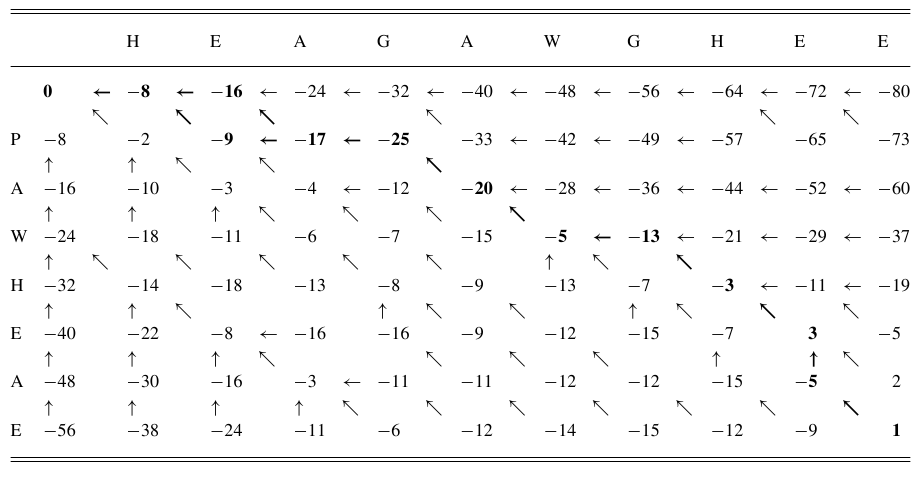
\includegraphics[width=15.1cm,keepaspectratio]{dyn-problem.png}
          \caption{\label{dyn-problem}Alignment for exercise \ref{dyn-p1}}
        \end{center}
      \end{figure}



    \item Statistical significance of alignments. 

      You have aligned two sequences, of length $m = 300$ and $n = 100$;
      suppose $K = 0.1$ and $\lambda = 0.7$. If we want to carry out a
      statistical test with Type I error of 0.05 (i.e., where the
      probability of rejecting the null hypothesis, when it is true, is
      0.05), what should be the threshold for the score? (Hint: look at
      equations \ref{eq:es} and \ref{eq:px}, and of course the definition
      of Type I error).


        % Basado en p. 61 de Bodorovsky.



      \item Suppose now that the sequence of length $n = 100$ is compared
        against a database where there are 2000 sequences of length $m=300$
        each one. What would be the E-value for a given threshold $S$?
        What about the $P-value$?

        % Basado en 2.19 en Bodorovsky.

        We can in fact solve very easily a more general problem where the
        query (our sequence of length $n$) is done against a database of
        lengths $m_1, m_2, \ldots, m_d$. Our specific example above would
        be one where $d = 2000$, and $m_1 = \ldots = m_{2000} = 300$.


        A hint:
        \begin{itemize}
        \item From the definition of the $E-value$, the $E$ for the
          complete search is the sum of the $E$s from each individual
          search: $E = \sum_{d=1}^{d = 2000}E_i$. Now, substitute the
          expression for $E_i$ and see if you can arrive at a simple
          expression. 
        \end{itemize}

        % Do not forget to show this. Note errata with minus sign in Bodorovsk

%%% P-value = P(S_max \ge S) = 1 - exp ^{-E} = 1 - e ^{- \sum E_i} = 1
%%% - \prod e ^{-E_i} = 1 - \prod (1 - P_i)


        \item Go the the NCBI or to ExPASy and do a BLAST search. For
          instance, EPAS1 (Q99814). Change the database, so that you use
          progressively larger databases. What happens with the
          $E-value$ and the score? You should be able to predict the
          results before doing the exercise.



%         \item Align sequences \verb=MTADKEKKRSSSERRKEKSRD= and
%           \verb=DKEKRRSSSESSRRSSSASK= using BLAST (NCBI will work
%           here). From the summary, calculate by hand the $E-value$ and the
%           bit score. (Note: in the table from ``Search summary'', you want
%           the right column of values for Lambda and K, since those are the
%           ones used for gapped alignments).

% %% This is no longer (2013-01-23) giving the results it should, according
% %% to tutorial in NCBI:
% %% http://www.ncbi.nlm.nih.gov/BLAST/tutorial/Altschul-1.html#head9
% %% and to
% %% http://etutorials.org/Misc/blast/Part+III+Practice/Chapter+7.+A+BLAST+Statistics+Tutorial/7.1+Basic+BLAST+Statistics/.


%% Also, E = m * n * 2^(-S'), where S' is the bit score. I get the bit
%% score right, but not the E-value.



%% E = 0.11 * 21 * 20 * exp(-0.294 * 69) ## 7.15 e-08
%% bit score: (0.294 * 69 - log(0.11))/log(2) ## 32.45




%% These almost do work
%%  TADKEK vs. itself with crap (e.g., WWWWWWWWWWWWW) before, so they are
%%  slightly larger

%% WWWWWWWWWWWWWWWWWWWWWWWWWWWWWWWWWWWWWWWWWWWWWWWWWWWWWWWWWWWWWWWWWWWWWWWWWWWWWWWWWWWWWWWWWWWWWWWWWWWWWWWWWWWWWWWWWWWWWWWWWWWWWWWWWWWWWWWWWWWWWWWWWWWWWWWWWWWWWWWWWWWWWWWWWWWWWWWWWWWWWWWWWWWWWWWWWWWWWWWWWWWWWWWTADKEK
%% MMMMMMMMMMMMMMMMMMMMMMMMMMMMMMMMMMMMMMMMMMMMMMMMMMMMMMMMMMMMMMMMMMMMMMMMMMMMMMMMMMMMMMMMMMMMMMMMMMMMMMMMMMMMMMMMMMMMMMMMMMMMMMMMMMMMMMMMMMMMMMMMMMMMMMMMMMMMMMMMMMMMMMMMMMMMMMMMMMMMMMMMMMMMMMMMMMMMMMMMMMMMMMMMMMMMMMMMMTADKEK




%% H is a relative entropy measure for a scoreing matrix
%% H = - \sum_i \sum_j  q_ij \lambda S_ij
%% larger H means more info

%% http://etutorials.org/Misc/blast/Part+II+Theory/Chapter+4.+Sequence+Similarity/4.4+Target+Frequencies+lambda+and+H/

%%% I have not included the multiple alignment exercises from the Proyecto
%%% Docente. Nor the comments about BLAST or FASTA.




%%%%%%%%%%%%%%%%%%%%%% My email with NCBI help staff

% From: matten@ncbi.nlm.nih.gov
% To: ramon.diaz@iib.uam.es, blast-help@ncbi.nlm.nih.gov
% Subject: Re: [blast-help] Expect value != m*n*2^(-S)?
% Flags: replied, seen
% Date: Tue 29 Jan 2013 00:38:27 CET
% Maildir: /Gmail/BM-13-2013

% Hello,

% I'm afraid that it is no longer possible to manually calculate the Expect
% values that you see from web blast searches. The most recent change is the
% use of a Finite Size Correction; please see the BLASTFeed (BLASTNews):

% http://www.ncbi.nlm.nih.gov/blast/Blast.cgi?CMD=Web&PAGE_TYPE=BlastNews[1]


% Best regards,
% Wayne

% <><>>><><><<<<><>>>>
% Wayne Matten, PhD
% NCBI User Services
% mattenw@mail.nih.gov



% -----Original Message-----
% From: Ramon Diaz Uriarte <ramon.diaz@iib.uam.es>
% Date: Monday, January 28, 2013 8:57 AM
% To: NLM/NCBI List blast-help <blast-help@ncbi.nlm.nih.gov>
% Subject: [blast-help] Expect value != m*n*2^(-S)?

% >
% >Dear Friends,
% >
% >For a class I am teaching, I am trying to replicate some calculations of E
% >values as explained, for instance, in
% >http://www.ncbi.nlm.nih.gov/BLAST/tutorial/Altschul-1.html#head3,[2]
% >
% >but the E-values reported by BLAST (as of today) do not agree with
% >those I compute. This is an example (the ID is GCY8D5Y8113):
% >
% >- we align (with default parameters) these two sequences:
% >
% >MTADKEKKRSSSERRKEKSRD
% >
% >DKEKRRSSSESSRRSSSASK
% >
% >
% >- The values for Lambda and K are 0.294 and 0.11 respectively.
% >
% >- Effective search space = 420 = n*m = 21 * 20
% >
% >- The bit score is: 32.5
% >
% >
% >E = 420 * 2 ^ (-32.5) = 6.9e-8
% >
% >but that differs from the reported value of 2e-09.
% >
% >
% >Note that the bit score and the score, lambda, and K do seem to make
% >sense, since I can get the bit score from the raw score as
% >
% >(lambda * S - ln K)/ln 2
% >
% >
% >
% >(0.294 * 69 - ln 0.11)/ln 2 = 32.45
% >
% >
% >
% >****
% >
% >I have repeated the above changing the sequences (for instance, using much
% >larger sequences and much shorter ones, using sequences that lead to
% >ungapped alignments), changing the default parameters, using other
% >substitution matrices, using no compositional adjustments, etc, etc, and I
% >can never reproduce the Expect value; my computed values seem to always be
% >about one to two orders of magnitude larger. (And I think this did not
% >happen about a year ago).
% >
% >What am I doing wrong?
% >
% >
% >Best,

\end{enumerate}



\subsection{Post-exercises: An example that no longer works}\label{nolonger}

This is an example of how we need to pay to attention to detail, and how
doing things by hand helps us question assumptions (or realize our
assumptions were wrong). This also shows that, often, asking the original
authors or help staff can really help sort out a problem.


This exercise used to work just fine:

\begin{itemize}
\item Align sequences \verb=MTADKEKKRSSSERRKEKSRD= and
  \verb=DKEKRRSSSESSRRSSSASK= using BLAST (NCBI will work
  here). From the summary, calculate by hand the $E-value$ and the
  bit score. (Note: in the table from ``Search summary'', you want
  the right column of values for Lambda and K, since those are the
  ones used for gapped alignments).

\end{itemize}


However, since at least 2013-01-23, that does not give the results it
should according to tutorial in NCBI:
\Burl{http://www.ncbi.nlm.nih.gov/BLAST/tutorial/Altschul-1.html\#head9}
and to
\Burl{http://etutorials.org/Misc/blast/Part+III+Practice/Chapter+7.+A+BLAST+Statistics+Tutorial/7.1+Basic+BLAST+Statistics/.}

Note that we can get the bit score right, but not the E-value. So the
problem is in computing the E-value.
\begin{verbatim}
E = 0.11 * 21 * 20 * exp(-0.294 * 69) ## 7.15 e-08
bit score: (0.294 * 69 - log(0.11))/log(2) ## 32.45
\end{verbatim}



So????


I wrote the help desk at the NCBI. This is the answer (with my original
email below):

{\small
\begin{verbatim}
From: matten@ncbi.nlm.nih.gov
To: ramon.diaz@iib.uam.es, blast-help@ncbi.nlm.nih.gov
Subject: Re: [blast-help] Expect value != m*n*2^(-S)?
Flags: replied, seen
Date: Tue 29 Jan 2013 00:38:27 CET
Maildir: /Gmail/BM-13-2013

Hello,

I'm afraid that it is no longer possible to manually calculate the Expect
values that you see from web blast searches. The most recent change is the
use of a Finite Size Correction; please see the BLASTFeed (BLASTNews):

http://www.ncbi.nlm.nih.gov/blast/Blast.cgi?CMD=Web&PAGE_TYPE=BlastNews


Best regards,
Wayne

<><>>><><><<<<><>>>>
Wayne Matten, PhD
NCBI User Services
mattenw@mail.nih.gov



-----Original Message-----
From: Ramon Diaz Uriarte <ramon.diaz@iib.uam.es>
Date: Monday, January 28, 2013 8:57 AM
To: NLM/NCBI List blast-help <blast-help@ncbi.nlm.nih.gov>
Subject: [blast-help] Expect value != m*n*2^(-S)?

>
>Dear Friends,
>
>For a class I am teaching, I am trying to replicate some calculations of E
>values as explained, for instance, in
>http://www.ncbi.nlm.nih.gov/BLAST/tutorial/Altschul-1.html#head3,
>
>but the E-values reported by BLAST (as of today) do not agree with
>those I compute. This is an example (the ID is GCY8D5Y8113):
>
>- we align (with default parameters) these two sequences:
>
>MTADKEKKRSSSERRKEKSRD
>
>DKEKRRSSSESSRRSSSASK
>
>
>- The values for Lambda and K are 0.294 and 0.11 respectively.
>
>- Effective search space = 420 = n*m = 21 * 20
>
>- The bit score is: 32.5
>
>
>E = 420 * 2 ^ (-32.5) = 6.9e-8
>
>but that differs from the reported value of 2e-09.
>
>
>Note that the bit score and the score, lambda, and K do seem to make
>sense, since I can get the bit score from the raw score as
>
>(lambda * S - ln K)/ln 2
>
>
>
>(0.294 * 69 - ln 0.11)/ln 2 = 32.45
>
>
>
>****
>
>I have repeated the above changing the sequences (for instance, using much
>larger sequences and much shorter ones, using sequences that lead to
>ungapped alignments), changing the default parameters, using other
>substitution matrices, using no compositional adjustments, etc, etc, and I
>can never reproduce the Expect value; my computed values seem to always be
>about one to two orders of magnitude larger. (And I think this did not
>happen about a year ago).
>
>What am I doing wrong?
>
>
>Best,

\end{verbatim}
}

Except for writing the help desk at NCBI, the only other things that would
have helped me were:
\begin{itemize}
\item Looking at the source code.
\item Keeping track of the changes in the program (the NEWS file and
  related pieces of information); this is something I do not do with BLAST
  (but yes with other software).
\end{itemize}






\clearpage
\section{Hidden Markov Models}\label{HMM}


\subsection{Introduction to Hidden Markov Models}\label{introhmm}

Hidden Markov Models (HMMs) are a very widely used modeling tool. In
bioinformatics, they are used for gene finding, multiple alignment and
description of protein family profiles, protein domain discrimination,
detection of copy number changes in genomic DNA, identification of
chromatin states, etc, etc, etc. We will spend a few pages on them. 



Start by reading the (third!) tutorial by Eddy,  ``What is a hidden
Markov Model'', in \textit{Nature biotechnology} \citep{Eddy2004a}.

If you know R, there is a small script (\texttt{hmm-eddy.R}) that repeats
some of the calculations in the paper (this is just a quick, step-by-step
example; this is not the proper way to code or analyze an HMM!).




Then, take a look at Krogh's chapter ``An introduction to Hidden
Markov Models for Biological Sequences'' \citep{Krogh1998}; read very
quickly (or skip entirely) section 4.4.


Finally, read section 10.3 of \citet{Higgs-Attwood}. I have included it in
Moodle, together with section 10.2 and 10.4. 10.2 is included only as
reference to some equations; section 10.4 is included for completeness,
and most of it should be fairly easy after reading Krogh. Make sure you
understand what they refer to, in p.~238, when they comment the
differences between M0-M1, M1-M1, etc.




% \red{FIXME: zz: algo de markov models? see Cristianin and Hahn, p. 8 y 9
%   (p. 28 y 29 del PDF). S�, poner estas dos p�ginas.}
% Y ver tb. cap�tulo 4 de Cristianin and Hahn, if el tutorial no es enough
% de Krough.









A few comments; more details on the algorithms in the next subsection.

\begin{itemize}
\item The tutorial by \cite{Krogh1998} mentions pseudocounts (p.\
  10). Note that this is a very common technique, not restricted to HMMs,
  nor to multiple alignments. Adding 1 is also known as Laplace's rule
  (and this was mentioned in BM-1; see p.\ 16 of the document ``An
  introduction to bioinformatics'').

\item \cite{Krogh1998}, in p.\ 12 to 13 (footnote 1 p.\ 13) is referring
  to estimating the parameters of the HMM using what is often called
  ``Viterbi training'' \citep[e.g. p. 64 in][]{Durbin1998}. This is also
  what \citet{Higgs-Attwood} are referring to in p.\ 237 (left
  column). However, ``Viterbi training'' performs less well than
  Baum-Welch (we explain Baum-Welch below, in section \ref{baum-welch}).

\item In the chapter by \citet{Higgs-Attwood} there are two errata in
  Fig.~10.2: arrows for $r_{B0}$ and $r_{0E}$ should be pointing to the right.

\item The examples in p.\ 240--241 of \citet{Higgs-Attwood} illustrate a
  key feature of building HMMs: choosing the topology of an HMM needs to
  be done very carefully, attending at the specific biological details and
  constraints of the problem. As \citet[][p.~68]{Durbin1998} emphasize,
  the idea of building a very complicated model to allow it to ``find out
  for itself'' rarely works.

\end{itemize}





\subsection{Viterbi, forward, backward, and all that}
\label{sec:viterbi-forw-backw}


There are four basic questions with HMMs:

\begin{itemize}
\item What is the most probable state path (i.e., path of hidden states)
  given an observed sequence?

\item What is the probability of a given observed sequence?

\item What is the posterior probability of a state $k$ at a time $i$?

\item How can we learn the parameters (transition and emission functions)
  for an HMM, given observed sequences?
\end{itemize}


We will use the \textbf{notation}:
\begin{description}
\item[The state path (the path over the hidden states):] $\pi$
\item[The observed sequence:] $x$. The i-th element is $x_i$, and the
  complete sequence goes from $1, \ldots,L$.
\item[Emission function:] $e_k(b)$ is the probability that symbol $b$
  (e.g., nucleotide A) is seen when we are in state $k$. Soon we will see
  the expression $e_k(x_i)$ which means the probability that
  we see the symbol for the i-th observation ($x_i$) emitted.
\item[Transition function:] We will write $a_{kl}$ for the probability
  that we go from state $k$ to state $l$. 

  We will use $a_{0k}$ for the transition from the ``begin state'' to the
  state $k$; this can be thought of as the probability of starting in
  state $k$. This was already in the tutorial by \cite{Eddy2004a} as
  ``Start'' in Figure 1 (and there $a_{0E} = 1$).  Likewise, $a_{k0}$ is
  the transition from $k$ to the ``end state''. In the tutorial, there was
  only one transition to the end state, with $a_{I0} = 0.1$. Yes, using
  $0$ for both the end and start states can seem confusing, but here we
  follow \cite{Durbin1998}.
\item We will index hidden states with $k$, going from $1,\ldots,M$ and
  the symbols of the alphabet (e.g., the nucleotides) with $b$, going from
  $1,\ldots,S$. 
\end{description}


Here are a few notes about each one of these questions.

\subsection{Viterbi: the most probable state path}
\label{sec:viterbi}


We want to find the \textbf{most likely path} given that we have observed
a sequence. The Viterbi algorithm does this. This problem is also called
(from its roots in speech recognition) \textbf{decoding}. 


Viterbi gives us
\begin{equation}
  \label{eq:viterbi}
  \pi^* = \underset{\pi}{\mbox{argmax}}\ P(x,\pi) = \underset{\pi}{\mbox{argmax}}\ P(\pi|x)
\end{equation}

So we are finding the most probable path. (Note that \cite{Higgs-Attwood}
refer to the likelihood, but this is not a likelihood.)


%% Add slide 10 of Ruzzo


Note, however, that the most probable state path is not the same as the
sequence of most probable states. We will return to this shortly (\ref{vit.ne.most-probable-state})


We do not need to examine all possible sequences. We can find this path
recursively, using dynamic programming.  We define $v_l(i)$ as the
probability of the most probable path emitting $x_1, x_2, \ldots, x_i$ and
ending in state $l$. We can find $v_l(i+1)$ recursively as:
\begin{equation}
  \label{vit1}
  v_l(i+1) = e_l(x_{i+1})\ \underset{k}{\max}(v_k(i)a_{kl})
\end{equation}
Make sure you understand the terms of that expression. This expression is
analogous to $S(i,j)$ in dynamic programming for sequence alignment (e.g.,
see equation \ref{eq:DP} in page \pageref{eq:DP}). 


We prepare a table, with $L$ columns (the observations) and $M$ rows (the
number of hidden states) and fill it up recursively as follows
\citep[from][p.~56]{Durbin1998}


\vspace*{5pt}
\setlength\fboxsep{0pt}
\setlength\fboxrule{0.5pt}
\fbox{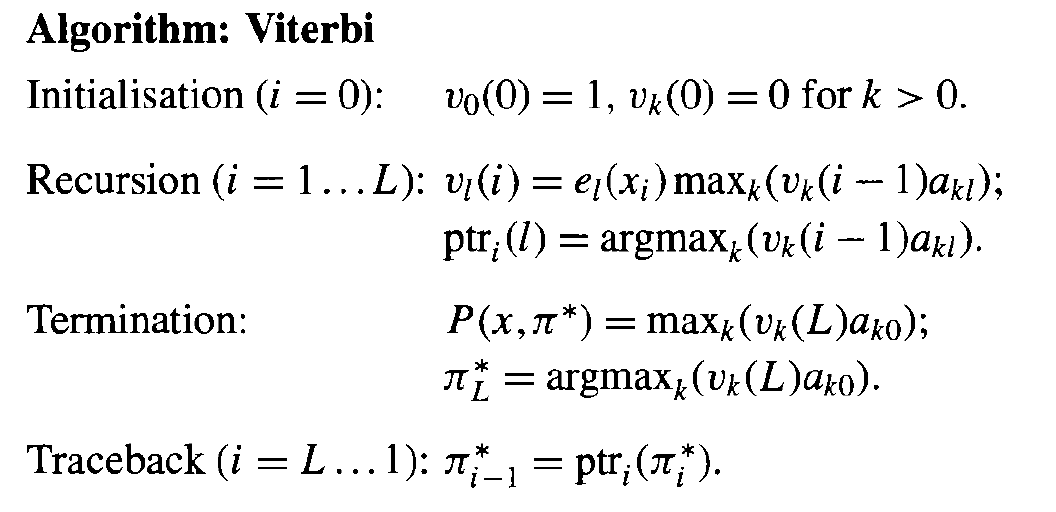
\includegraphics[width=10.1cm,keepaspectratio]{viterbi-algo-durbin.png}
}

In the above, $ptr$ means ``pointer'', so we can traceback.

Minor point: the ``Termination'' step with $a_{k0}$ is there in case that
an end step is explicitly modeled. Otherwise, the $a_{k0}$ would disappear.


That's it! 


The following slide from the presentation on HMMs
by L.~Ruzzo
(\Burl{http://www.cs.washington.edu/education/courses/cse527/09au/}),
p. 29 can help:


\vspace*{5pt}
\setlength\fboxsep{0pt}
\setlength\fboxrule{0.5pt}
\fbox{
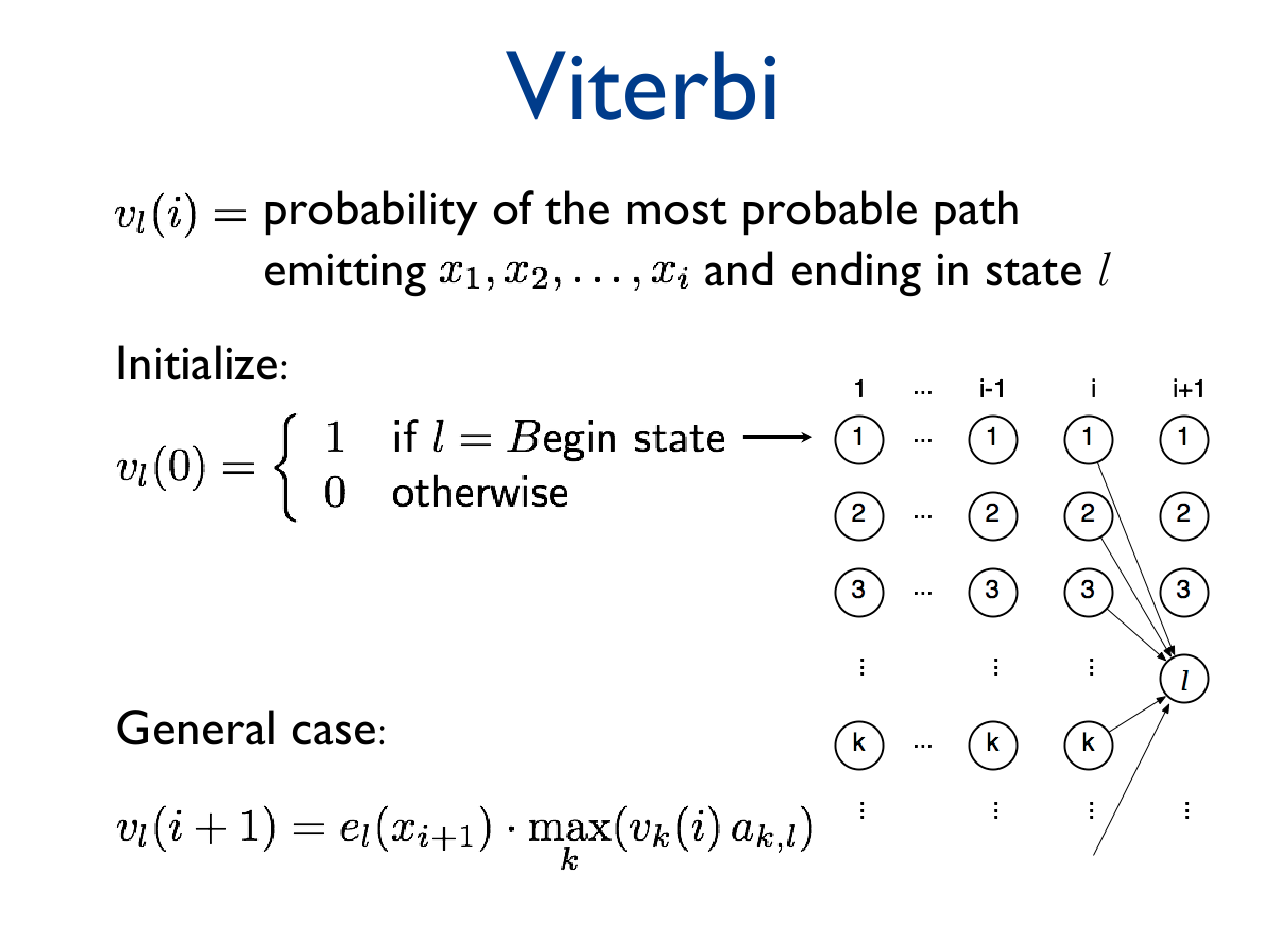
\includegraphics[width=14.1cm,keepaspectratio]{viterbi-ruzzo0.png}
}





%% Think about simple cases with initial run, L = 1, etc.
%% And why is e_l(x_i) not inside the maximization?

\clearpage
Just to give a very simple example, I copy from the presentation on HMMs
by L.~Ruzzo
(\Burl{http://www.cs.washington.edu/education/courses/cse527/09au/}), pp.\
30 and 31 (he also provides an Excel spreadsheet you can play with):

\vspace*{5pt}
\setlength\fboxsep{0pt}
\setlength\fboxrule{0.5pt}
\fbox{
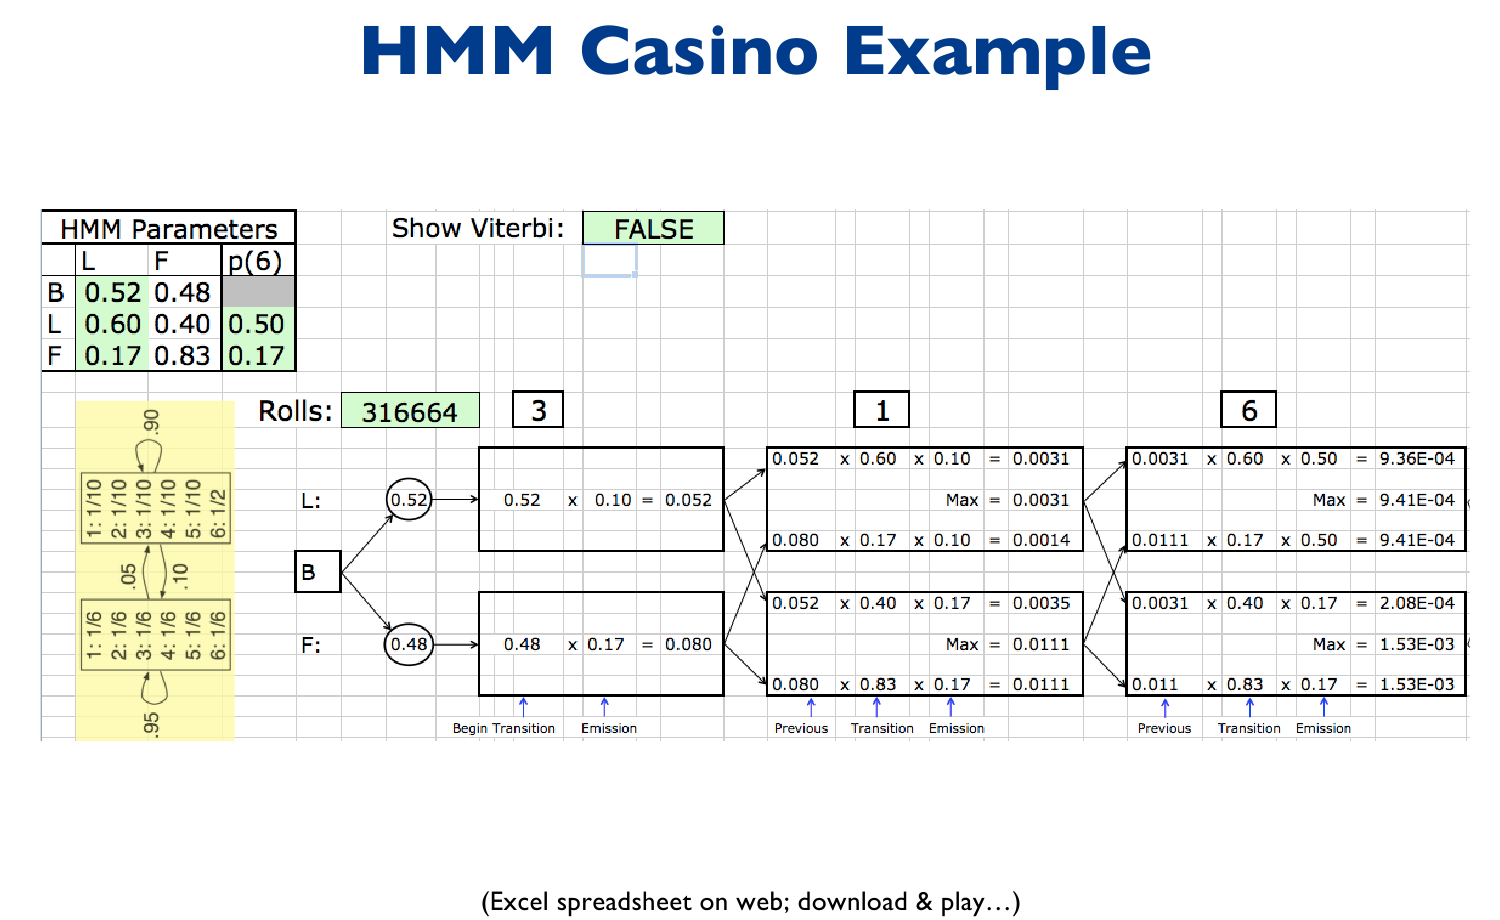
\includegraphics[width=15.1cm,keepaspectratio]{viterbi-example-ruzzo1.png}
}

\vspace*{4pt}
\fbox{
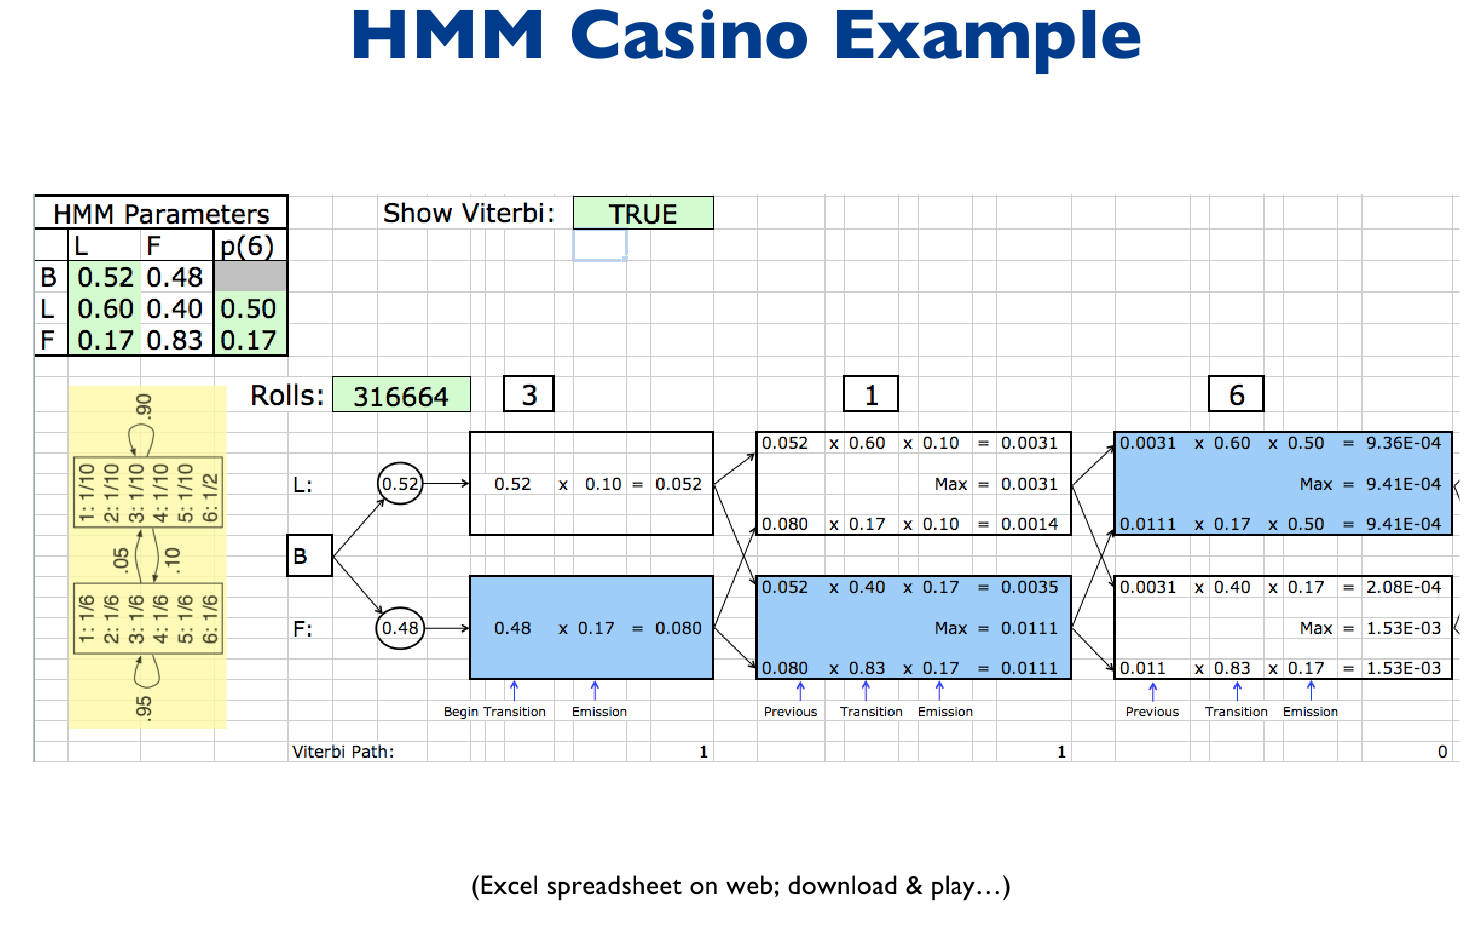
\includegraphics[width=15.1cm,keepaspectratio]{viterbi-example-ruzzo2.png}
}



\subsubsection{Viterbi: using logs}
\label{sec:viterbi:-using-logs}
We are multiplying many small numbers (probabilities and emission
functions), so in ``real life'' we will run into underflow problems. A
common procedure to prevent this problem is to use logarithms (and,
instead of multiplying probabilities, sum logs of probabilities). 

We can do this with Viterbi as follows \citep[][p.~77]{Durbin1998}: lets
use a tilde for the parameters after taking the log, so we would have
$\tilde{a}_{kl} = \log a_{kl}$, and call $V$ the $v$ after taking the
log. The recursion equation \ref{vit1} would then be:
\begin{equation}
  \label{vitlog}
  V_l(i+1) = \tilde{e}_l(x_{i+1})+\underset{k}{\max}(V_k(i) + \tilde{a}_{kl})
\end{equation}







\subsection{Forward algorithm: probability of a sequence}
\label{forw-algor-prob}

We want to know
\begin{equation}
  \label{forward1}
  P(x) = \sum_{\pi} P(x,\pi)
\end{equation}
Again, no need to enumerate all paths. We can use dynamic programming. Let
\begin{equation}
  \label{forward2}
  f_k(i) = P(x_1,x_2,\ldots,x_i,\pi_i = k)
\end{equation}
be the probability of being in state $k$ having observed the first $i$
characters of $x$ (i.e., $x_1,x_2,\ldots,x_i$). So we go forward, from
$x_1$ up to, and including, $x_i$.

For each one of the states, $k$, we want to find $f_k(L)$, or the
probability of having observed all of the sequence and be in state $k$.





The recursion equation is:
\begin{equation}
  \label{forward3}
  f_l(i + 1) = e_l(x_{i+1}) \sum_k f_k(i) a_{kl}.
\end{equation}

Make sure you understand why that makes sense.


The algorithm then is just \citep[from p.~58 in][]{Durbin1998}:

\vspace*{5pt}
\setlength\fboxsep{0pt}
\setlength\fboxrule{0.5pt}
\fbox{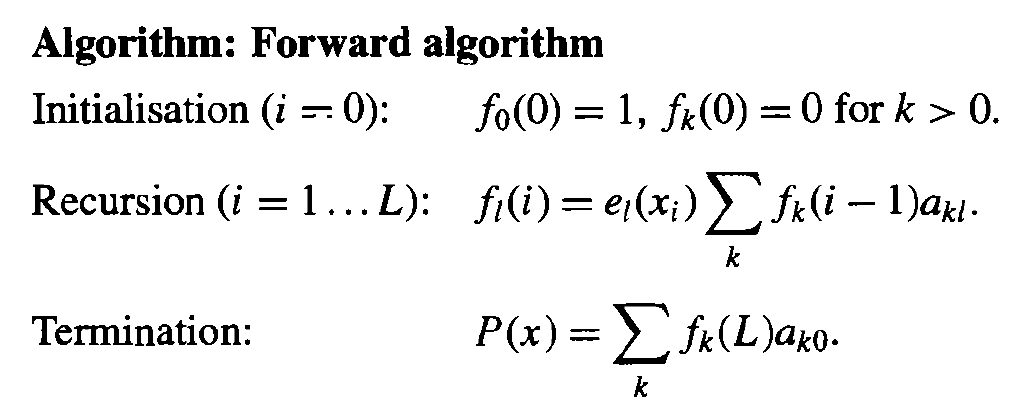
\includegraphics[width=10.1cm,keepaspectratio]{forward-algo-durbin.png}
}


Notes:

\begin{itemize}
\item At least initially, you might also want to explicitly prepare a
  table with $L$ columns and $M$ (or $M + 1$, where the extra is for the
  initial state 0) rows.
\item We initialize $f_0(0) = 1$, as that is the probability that we are
  in the start state and have not observed any elements of the sequence
  (or observed 0 elements of the sequence). All the rest have to be 0.
\item The termination is the probability that we have observed the
  complete sequence ($f_k(L)$) and we are in the end state (and thus the
  multiplication by $a_{k0}$). 
\item Essentially, we are just saying that the probability of a sequence
  is the sum of all the paths that can produce that sequence. In contrast,
  with Viterbi we used $\max$ instead of $\sum$.
\item The presentation by Dewey and Craven
  \Burl{http://www.biostat.wisc.edu/bmi576/lectures/HMMs-1.pdf} uses $P(x)
  = f_N(L) = \sum_k f_k(L) a_{kN}$. This notation might help, and might be
  handy latter (section \ref{baum-welch}). Note that they use $a_{kN}$
  which is, arguably, much clearer than $a_{k0}$ to denote the transition
  from $k$ to the end state.
\end{itemize}



The following figures might help to understand what is happening. They all
come from the course
\Burl{http://www.biostat.wisc.edu/bmi576/syllabus.html}, by M.~Craven.


The first shows the calculation of the probability of a given sequence and
path (pp.\ 4 and 5 of
\Burl{http://www.biostat.wisc.edu/bmi576/lectures/HMMs-1.pdf}).This
is also an interesting example, because not all transitions are allowed
(do you see that?). Note that we already did similar calculations when
using R to repeat the calculations in Eddy's tutorial
(\texttt{hmm-eddy.R}, section \ref{introhmm}).

\vspace*{5pt} \setlength\fboxsep{0pt}
\setlength\fboxrule{0.5pt} \fbox{
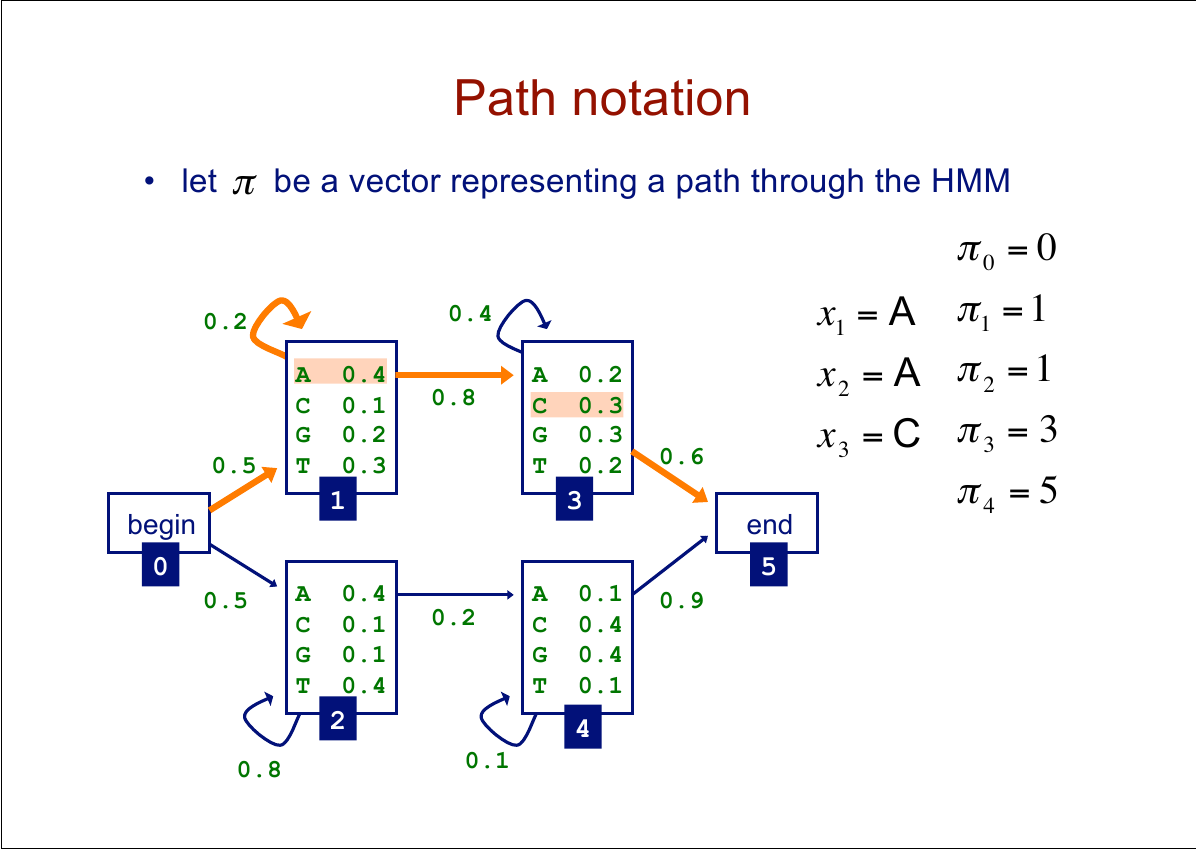
\includegraphics[width=14.1cm,keepaspectratio]{prob-seq-craven-1.png}
}

\vspace*{5pt} 
\setlength\fboxsep{0pt} \setlength\fboxrule{0.5pt} \fbox{
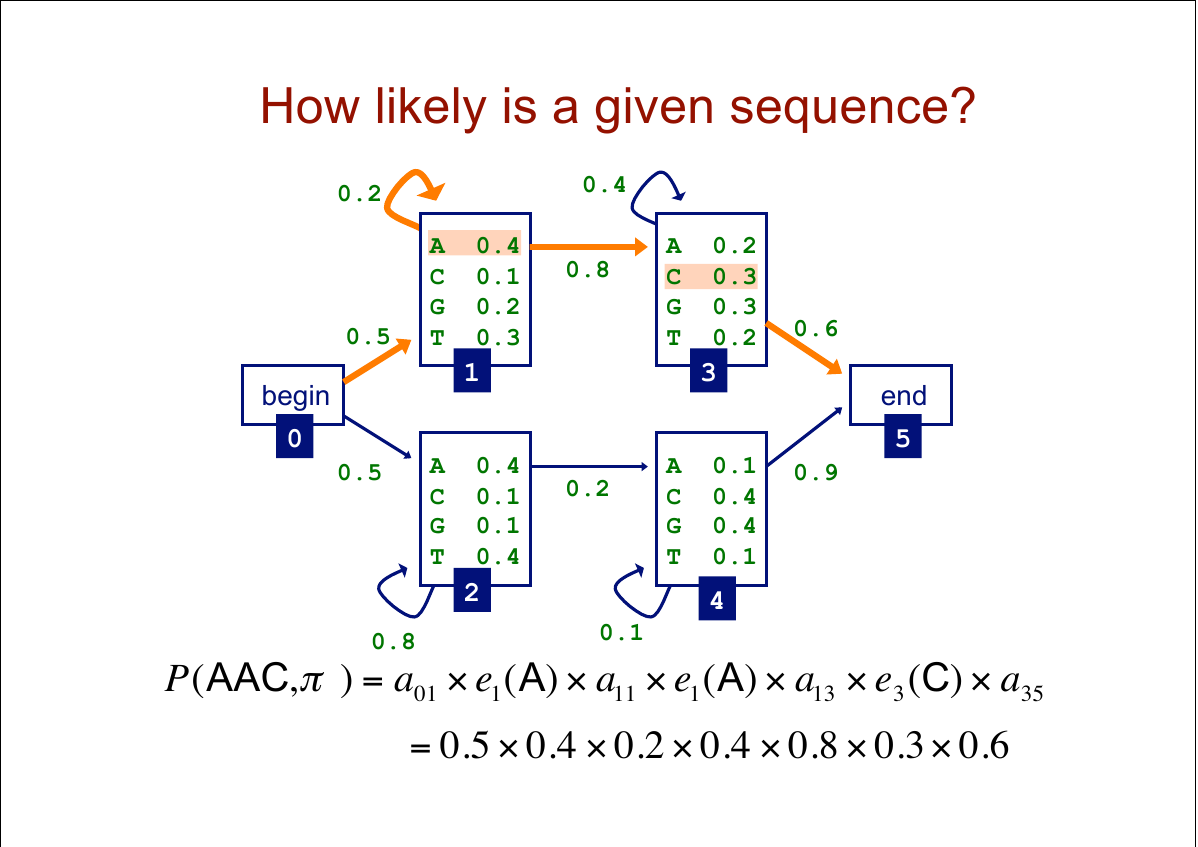
\includegraphics[width=14.1cm,keepaspectratio]{prob-seq-craven-2.png}
}


\clearpage
The next show a very simple example of using the forward algorithm, and
are from pages 9 and 10 of the PDF
\Burl{http://www.biostat.wisc.edu/bmi576/lectures/HMMs-1.pdf}


\vspace*{5pt} 
\setlength\fboxsep{0pt} \setlength\fboxrule{0.5pt} \fbox{
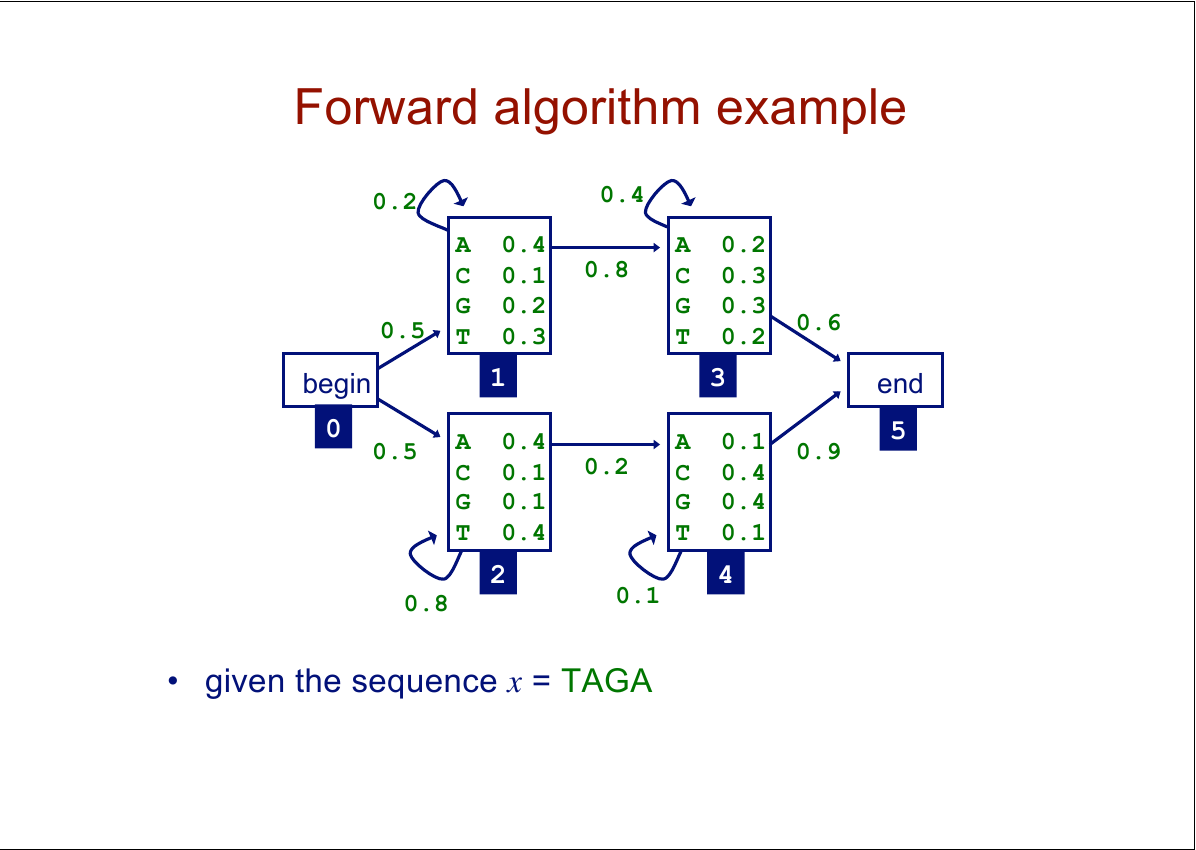
\includegraphics[width=14.1cm,keepaspectratio]{forward-craven-1.png}
}

\vspace*{4pt}
\fbox{
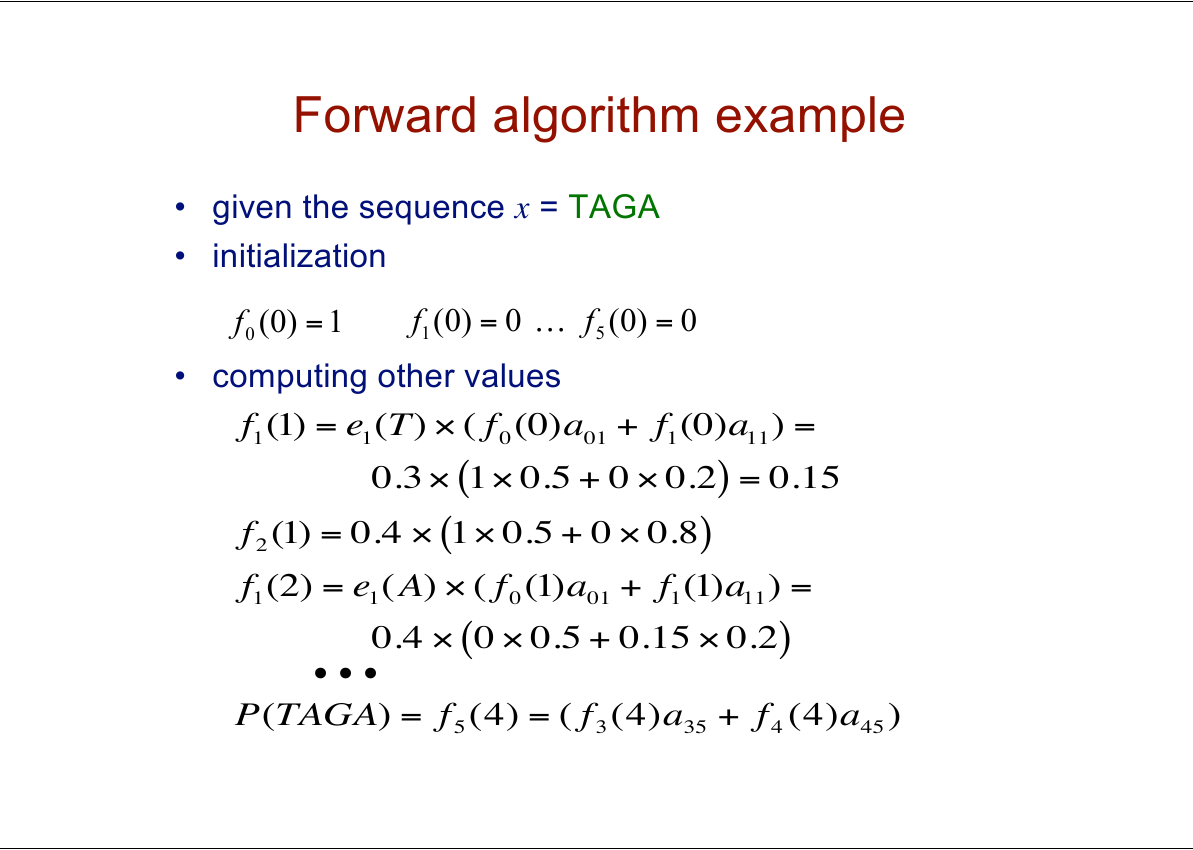
\includegraphics[width=14.1cm,keepaspectratio]{forward-craven-2.png}
}

\vspace*{25pt}








The above calculations (using probabilities) are not the best for ``real
stuff'', as we can run into underflow problems, similar to what happened
with Viterbi. We will not deal with these problems here, but there are
workarounds (though more cumbersome than for Viterbi).

\clearpage
\subsection{Backward algorithm: posterior probability of a state}
\label{sec:backw-algor-post}


We want to find $P(\pi_i = k|x)$ and we know we can write
\begin{equation}
  \label{eq:bw1}
P(\pi_i = k|x) = \frac{P(x, \pi_i = k)}{P(x)}
\end{equation}
where $P(x)$ we already found in the previous section. What about the
numerator?

\begin{eqnarray}
  \label{eq:bw2}
  P(x, \pi_i = k) &=& P(x_1, \ldots, x_i, \pi_i = k)
  P(x_{i+1},\ldots,x_L|x_1, \ldots, x_i, \pi_i = k) \\
  &=& P(x_1, \ldots, x_i, \pi_i = k) P(x_{i+1},\ldots,x_L|\pi_i = k) 
\end{eqnarray}
(make sure you understand why the above expressions are correct).


The first term is $f_k(i)$, as found in the previous section. The second
term we will call $b_k(i)$ so
\begin{equation}
  \label{eq:bw3}
  b_k(i) = P(x_{i+1},\ldots,x_L|\pi_i = k) 
\end{equation}
It is similar to the forward variable, but we go backwards, starting from
the end of the sequence, and arriving at $\pi_i$.


There is a recursive algorithm for finding $b_k$, which I copy from
\citet[][p.~59]{Durbin1998}:

\vspace*{5pt}
\setlength\fboxsep{0pt}
\setlength\fboxrule{0.5pt}
\fbox{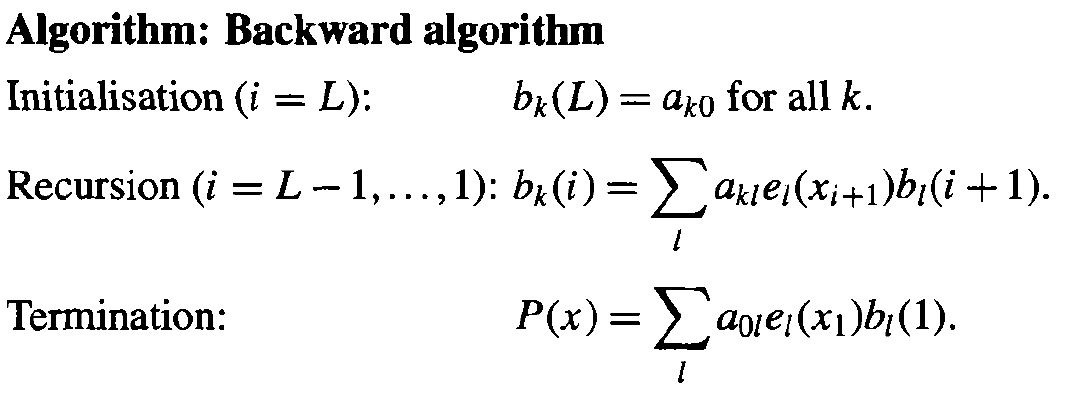
\includegraphics[width=10.1cm,keepaspectratio]{backward-algo-durbin.png}
}

(We have also a
``termination'' condition, but that is rarely used, because we often
already have $P(x)$ from the forward algorithm; of course, $P(x)$ from
this algorithm or from the forward one should be the same).



So now we can write
\begin{equation}
  \label{eq:bw4}
  P(\pi_i = k|x) = \frac{f_k(i)b_k(i)}{P(x)}
\end{equation}



Note: this is also called in many places ``posterior decoding'', but
beware of that term, as sometimes it is used with a slightly different
meaning. 


\clearpage
\subsubsection{A graphical view of backward vs.\  forward}

This comes from L.~Ruzzo's presentation on HMMs at 
(\Burl{http://www.cs.washington.edu/education/courses/cse527/09au/}), p.\
38 and 39:


\vspace*{5pt}
\setlength\fboxsep{0pt}
\setlength\fboxrule{0.5pt}
\fbox{
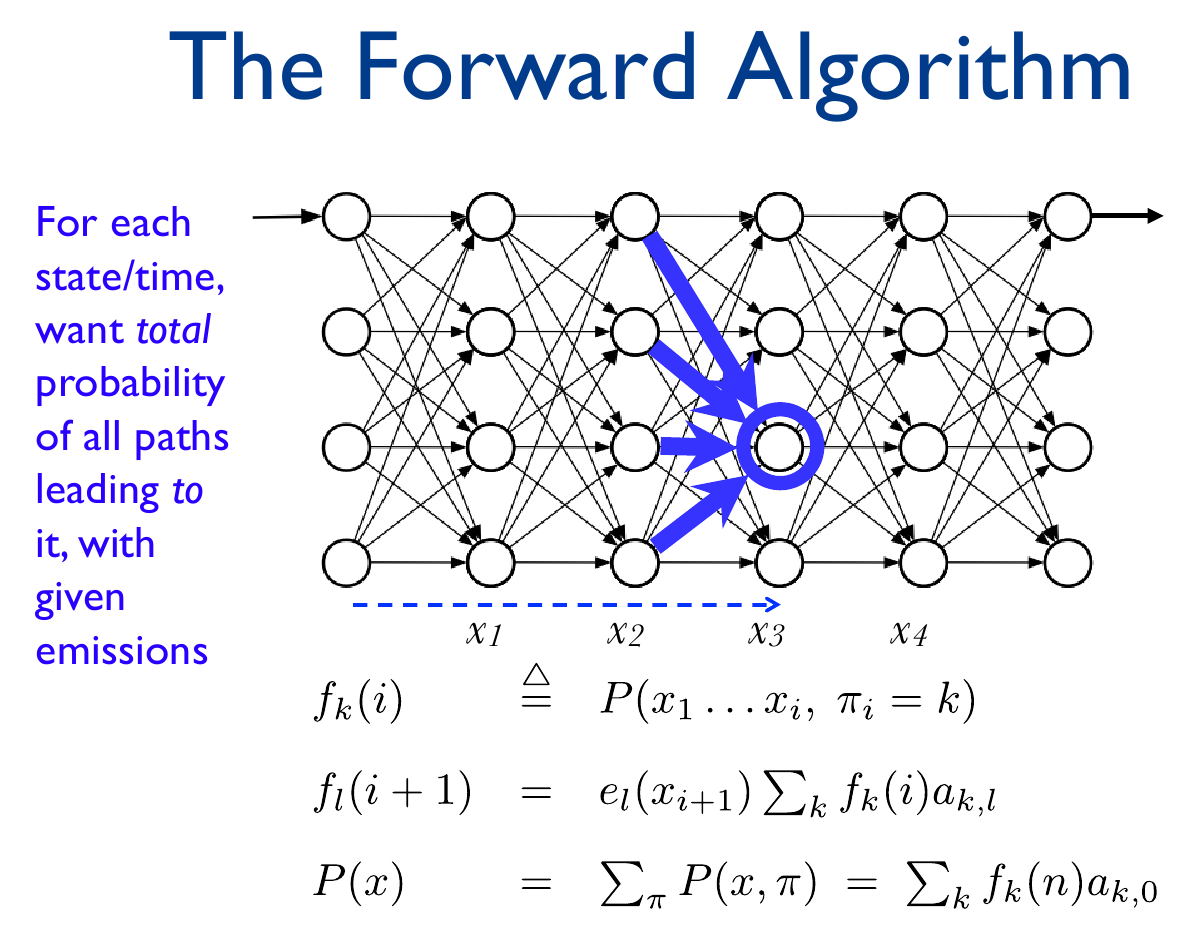
\includegraphics[width=12.1cm,keepaspectratio]{forward-ruzzo.png}
}

\vspace*{4pt}
\fbox{
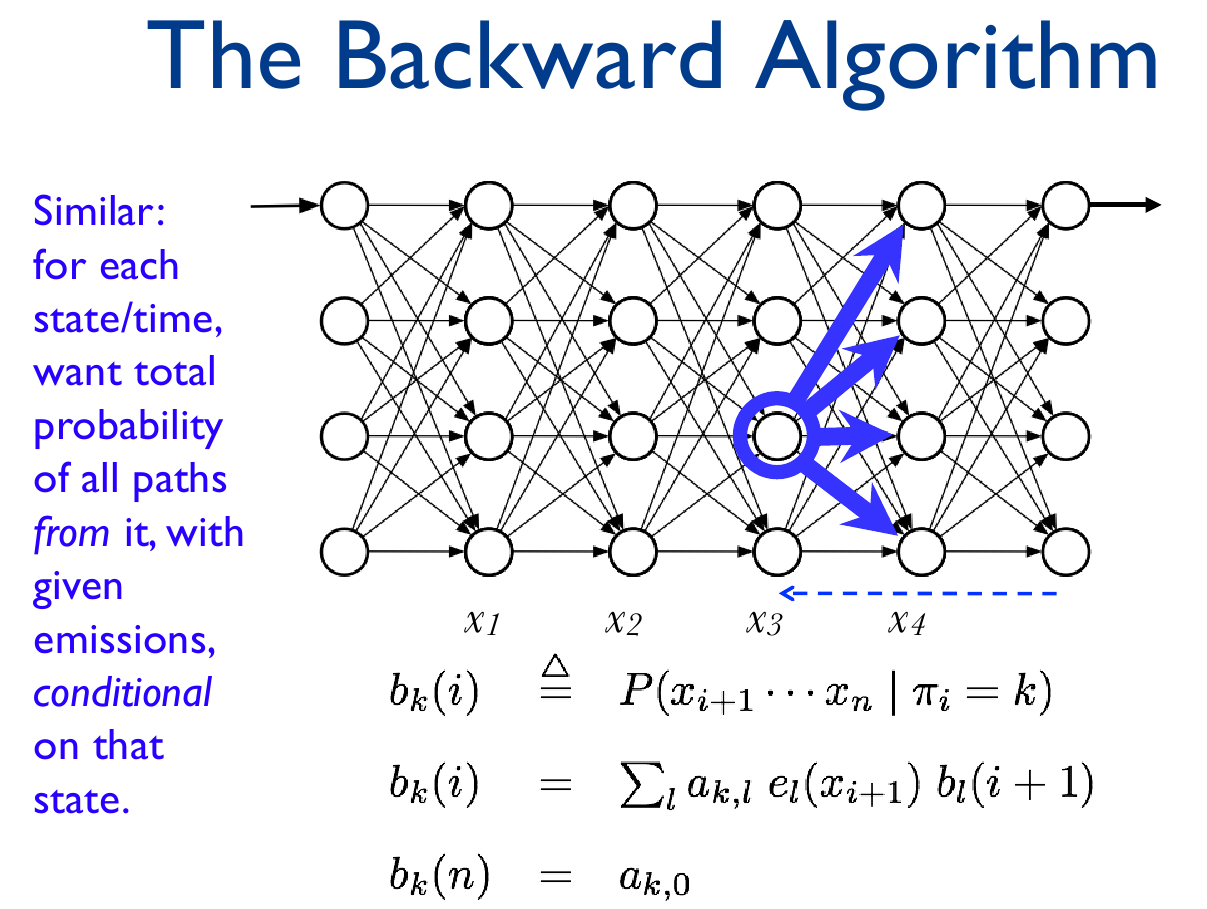
\includegraphics[width=12.1cm,keepaspectratio]{backward-ruzzo.png}
}






\subsubsection{Most probable state path vs.\ sequence of most probable states}
\label{vit.ne.most-probable-state}

The most likely state at step $i$ is given by
\begin{equation}
  \label{eq:mostlikely}
  \hat{\pi_i} = \underset{k}{\mbox{argmax}}\ P(\pi_i = k|x)
\end{equation}
but the sequence defined by all the $\hat{\pi_i}$ might not be the same as
that found by Viterbi (equation \ref{eq:viterbi}). In fact, it might not
even be a possible, legitimate path if not all transitions are allowed.


A simple illustration from the presentation by L.~Ruzzo on HMMs 
(\Burl{http://www.cs.washington.edu/education/courses/cse527/09au/}), p.\
34:

\vspace*{5pt}

\setlength\fboxsep{0pt}
\setlength\fboxrule{0.5pt}
\fbox{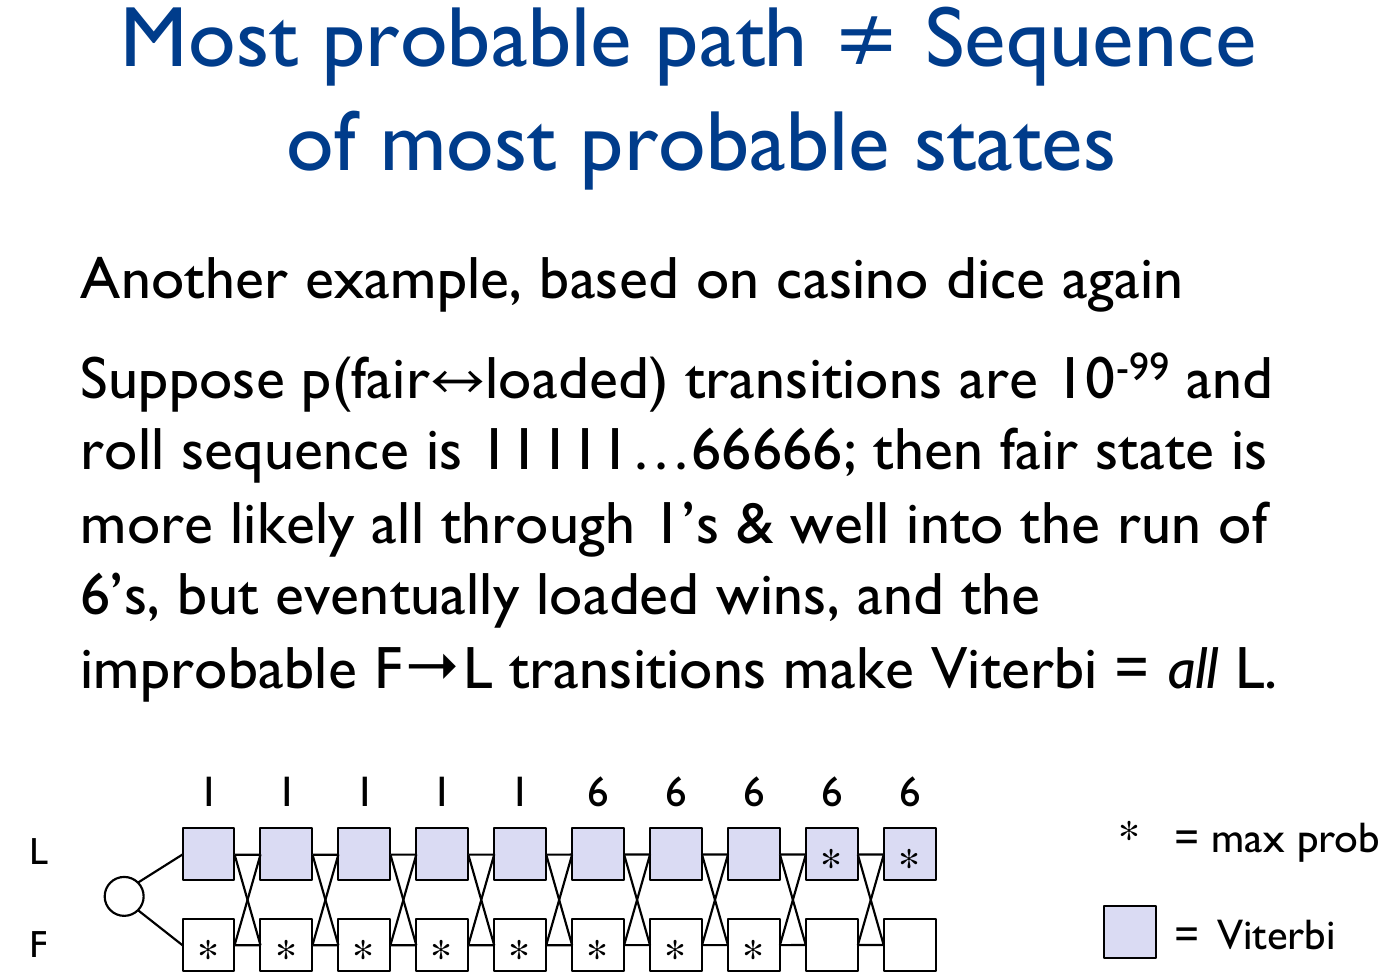
\includegraphics[width=15.1cm,keepaspectratio]{ruzzo-most-prob-path.png}
}
 % \begin{figure}[h!]
 %     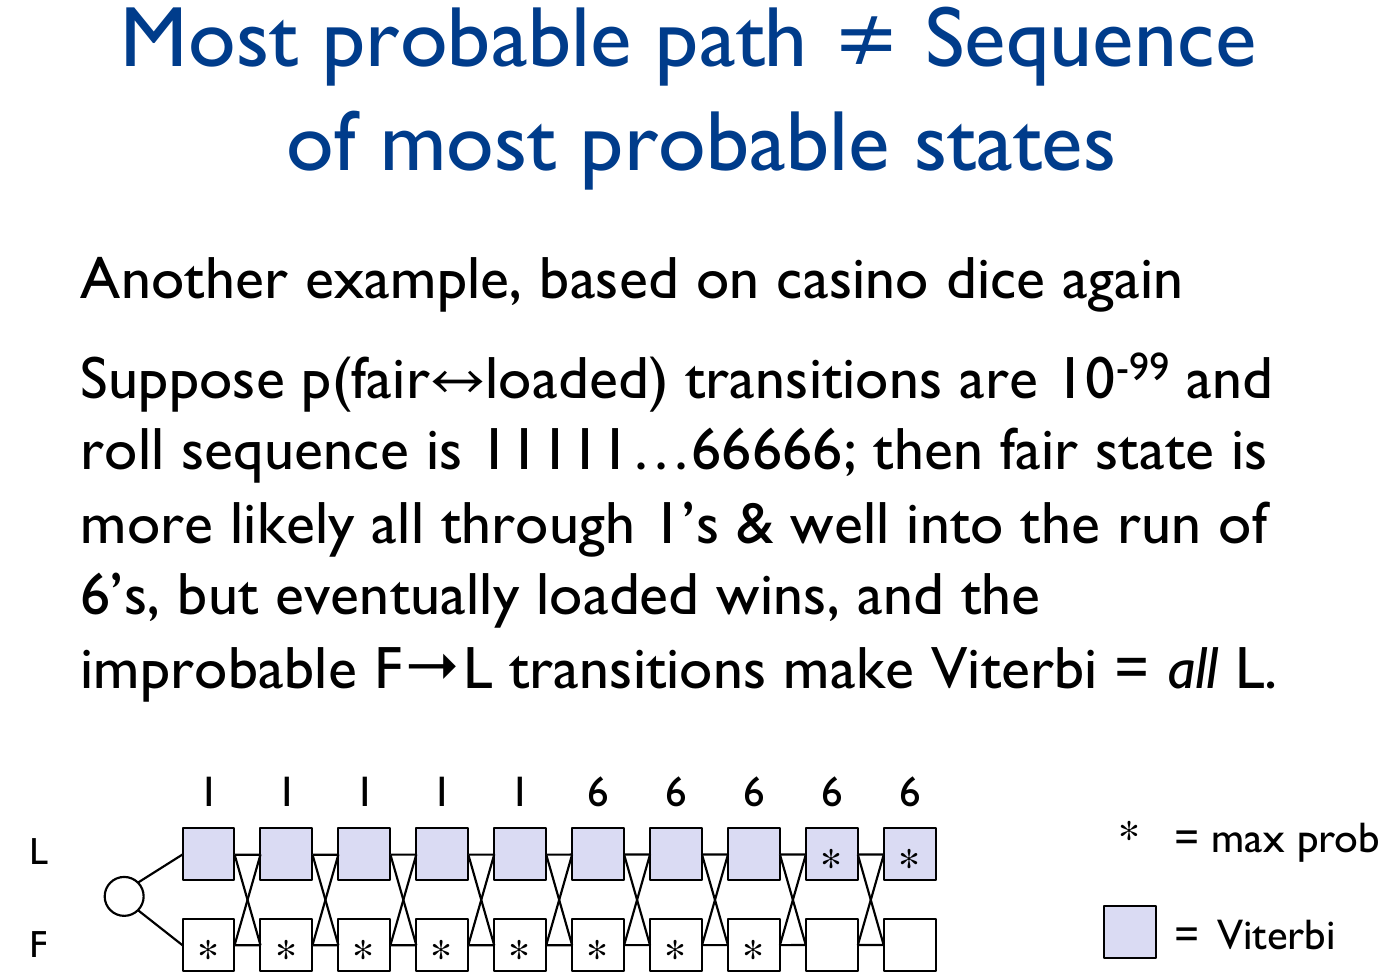
\includegraphics[width=15.1cm,keepaspectratio]{ruzzo-most-prob-path.png}
 % \end{figure}



\subsection{Learning the parameters}
\label{sec:learning-parameters}

(In what follows, we take topology as known).

\subsubsection{When the paths are known}
\label{sec:when-paths-are}
For one or more training samples we also know the true values of the
hidden variables. Thus, we know the paths, the $\pi$. We want to estimate
the parameters, $\theta$, which in our HMMs are the emission and transition
functions. This is immediate, and the maximum likelihood estimates
corresponds to the observed frequency in the data. You just need to count.


The expressions are\footnote{The expressions in \cite{Durbin1998} are
  written with a different notation for the sums, which might be
  confusing, even if simpler:
The expressions are
\begin{equation*}
  a_{kl} = \frac{A_{kl}}{\sum_{l'}A_{kl'}} %\label{mle-ao}
\end{equation*}
%and
\begin{equation*}
  e_k(b) = \frac{E_k(b)}{\sum_{b'}E_k(b')} %\label{mle-eo}
\end{equation*}}
\begin{equation}
  a_{kl} = \frac{A_{kl}}{\sum_{m=1}^{m=M}A_{km}} \label{mle-a}
\end{equation}
and
\begin{equation}
  e_k(b) = \frac{E_k(b)}{\sum_{s=1}^{s=S}E_k(s)} \label{mle-e}
\end{equation}
where $A_{kl}$ means the counts of the transitions from state $k$ to state
$l$ and $E_k(b)$ is the count of the number of times symbol $b$ is emitted
when in state $k$. And the denominators of each expression just count the
number of transitions from $k$ to all other states and the total number of
emissions while on state $k$.



% The expressions are
% \begin{equation}
%   a_{kl} = \frac{A_{kl}}{\sum_{l'}A_{kl'}} \label{mle-a}
% \end{equation}
% and
% \begin{equation}
%   e_k(b) = \frac{E_k(b)}{\sum_{b'}E_k(b')} \label{mle-e}
% \end{equation}


Often, in those expressions we would add pseudocounts, to avoid zero and
undefined probabilities.

\subsubsection{When the paths are unknown: Baum-Welch}
\label{baum-welch}


When the paths are unknown, we cannot directly use equations \ref{mle-a}
and \ref{mle-e}, since we do not know the hidden states. In addition, in
this case we often need not only learn the parameters, as before, but also
infer the true labels of the hidden states. In fact, in many (most?) cases
what we \textit{really} care about is the path, the hidden states.


There are a variety of approaches to solve this problem. We will discuss
here the Baum-Welch algorithm. However, as you read in
\cite{Higgs-Attwood} and \cite{Krogh1998}, there is also a procedure
called ``Viterbi training'', which is an iterative procedure, slightly
simpler than Baum-Welch, that uses the Viterbi algorithm; but Baum-Welch
is generally superior. And there are other approaches, for instance the
Bayesian approach used in \citet{Rueda2007}; or general optimization
techniques, etc.



\vspace*{18pt} Oh, before we get going: what are you supposed to know
from this section? No, I do not expect you to memorize the formulas. But
you should understand what the Baum-Welch algorithm is about. And you are
likely to find ``EM'' in many, many papers.
\vspace*{18pt}



%% In \cite{Zucchini2009}, the book by Zucchini and MacDonald, p. 63,
%% there is a very detailed explanation of the EM algor.


The Baum-Welch procedure is a special case of a more general procedure
called the \textbf{EM} algorithm, where EM stands for
``expectation-maximization''. The EM algorithm is often used in ``missing
data'' situations; our ``missing data'' are the labels or true values of
the hidden states, $\pi$\footnote{Some clustering methods (mixture models)
  are also estimated using EM because, as here, there are ``hidden
  variables'' (the cluster memberships of the samples)}.

The intuitive idea is to iterate between
these two steps (after initializing the values of $\theta$ ---$a$ and $e$):
\begin{enumerate}
\item Given an estimated set of parameters, $\theta$, calculate the
  \textit{expected} number of times each transition and emission is
  used. \textbf{E-step}

 % estimate the labels of the hidden
 %  states, $\pi$. \textbf{E-step}.
\item Recompute the values of $\theta$, so as to \textit{maximize} the
  likelihood. \textbf{M-step}.
\item Calculate the log-likelihood (to know whether or not to
  stop): $\log P(x|\theta)$. 
\end{enumerate}

The above iteration is continued until a predefined stopping criterion is
reached (e.g., successive iterations lead to only very minute changes in
the likelihood). However, beware that the convergence can be to local
optima, not necessarily the global optimum. This problem is especially
serious with very complex HMMs. There are some ways of trying to improve
your chances of finding the global optimum (the simplest is to start the
procedure from several different points).


\vspace*{10pt}
Why the above procedure? We said the Baum-Welch is a special case of the
EM algorithm. What we want to do, in general, is find the model that
maximizes the likelihood. We saw this already in section \ref{ML}, where
we used the expression 
\[\underset{\theta}{\mbox{argmax}}\ P(Data|\theta)\]
(equation \ref{eq:ML}). For brevity, now, we will write $x$ instead of
$Data$, i.e.,
\[\underset{\theta}{\mbox{argmax}}\ P(x|\theta)\]
but, now, there are ``missing data'', in our case the $\pi$.

With the EM we proceed iteratively. Suppose we have a set of initial
parameters, $\theta^0$. We want to obtain a new set of parameters,
$\theta^1$ so that the model improves (the likelihood increases). And then
repeat.  So we want to increase the likelihood as we go from $\theta^t$ to
$\theta^{t+1}$. To achieve this, a function is defined which is an average
of $P(x,\pi|\theta)$ over the distribution of $\pi$. This function is
often called $Q$ \citep[and that is how it is called in pp.~323--325
of][]{Durbin1998}\footnote{More precisely, Q is the expected value of the
  log-likelihood with respect to the conditional distribution of $\pi$
  given $x$ under the current estimate of the parameters $\theta^t$
  ---for instance, equation 11.31 in p.~323 of \citet{Durbin1998}}. What the general EM does is iterate between these
two steps:
\begin{itemize}
\item Calculate $Q$ given the current estimates of $\theta$,
  $\theta^t$. \textbf{E-step}.
\item Maximize $Q$ with respect to $\theta$ to obtain $\theta^{t+1}$. \textbf{M-step}
\end{itemize}

It turns out that with HMMs those two steps involve doing what we now explain in more detail.

\vspace*{10pt}







\paragraph{E-step: Expectation step}
\label{sec:expectation-step}

We want to obtain the expected values of $A$ and $E$. 

With an argument similar to the one we used for equation \ref{eq:bw2} we get:
\begin{equation}
  \label{eq:es1}
P(\pi_i = k, \pi_{i + 1} = l | x, \theta) = \frac{f_k(i) a_{kl} e_l(x_i +
  1) b_l(i + 1)}{P(x)}  
\end{equation}

What is the above? That is the probability of going from state $k$ to
state $l$ (given, of course, the observed $x$ and our current estimates of
the parameters). We want the expected value of $A_{kl}$, which we get by
summing over all training sequences (the $j$ index below) and over all
positions (the $i$):

\begin{equation}
  \label{eq:es2}
  A_{kl} = \sum_j \frac{1}{P(x^j)} \sum_i f_k^j(i) a_{kl} e_l(x_i^j +
  1) b_l^j(i + 1)
\end{equation}
and note that $P(x^j) = f_N^j(L)$ (see note in \ref{forw-algor-prob} for
explanation of $f_N$).


Similarly, we can find the expected value for $E$
\begin{equation}
  \label{eq:es3}
  E_k(b) = \sum_j \frac{1}{P(x^j)} \sum_{\{i|x_i^j=b\}} f_k^j(i) b_k^j(i)
\end{equation}
And what is the second $\sum$ over? Over all those positions where $b$ is
seen in the sequence $x^j$: we only want to sum when symbol $b$ is emitted
by hidden state $k$. (Look at equation \ref{eq:bw4}, and you'll see they
are very similar).

% , but here we are restricting the sum to those cases in
% which symbol $b$ is emitted).




So the expectation step involves:
\begin{enumerate}
\item Calculate $f_k(i)$ (with the forward algorithm).
\item Calculate $b_k(i)$ (with the backward algorithm).
\item Calculate $A_{kl}$ (equation \ref{eq:es2}). 
\item Calculate $E_k(b)$ (equation \ref{eq:es3}).
\end{enumerate}


\paragraph{M-step: Maximization step}
\label{sec:maximization-step}

The maximization step involves using whatever we have so far, in equations
\ref{mle-a} and \ref{mle-e}. It is finding the maximum likelihood
estimates of the parameters (that is why we use equations \ref{mle-a} and
\ref{mle-e}). 


For instance, write
\begin{equation}
  \label{eq:me1}
  \hat{a}_{kl} = \frac{\hat{A}_{kl}}{\sum_{m=1}^{m=M}\hat{A}_{k,m}}
\end{equation}
and likewise for $\hat{e}$.



\paragraph{Computing the log likelihood}
\label{sec:comp-log-likel}

We often have several sequences. Thus we do
\begin{equation}
  \label{eq:esloglik}
  \log P(x|\theta) = \sum_{x^j} \log P(x^j|\theta)
\end{equation}


\paragraph{Initialization}
\label{sec:initialization}

The initial parameters can be set to 0, or the values from the
pseudocounts, or to something else that might seem sensible.


\paragraph{The hidden states}
\label{sec:hidden-states}
The algorithm did its job, and we have our estimates of $\theta$,
$\hat{\theta}$. But we said that what we are often really interested in
are the hidden states, the $\pi_i$. So, now what?




\vspace*{15pt}

There is a worked out example, by hand, in pp.~12 and ff.\ of Craven's
presentation: \Burl{http://www.biostat.wisc.edu/bmi576/lectures/HMMs-2.pdf}.




\vspace*{20pt}




% \subsubsection{And the topology?}
% \label{sec:learning-topology}

% That is a different business.A few comments have been made above a




%% Write Mark Craven and ask for permission







% Good news: no need to read me anymore (for this part) ;-). We now use
% material from other people. 



\subsection{EXERCISES: HMMs}
\label{exerc-hmms}

\begin{enumerate}

\item Dynamic programming tables for HMMs.

  Suppose the model in Figure 1 of Eddy's HMM tutorial
  \cite{Eddy2004a}. You are given the sequence \verb=CTCTAGAGT=. Think
  about the dynamic programming table: there are a number of cells that
  you know you can fill with 0s. Which are those?

%% ojo con las del final. las dos ultimas columnas de E, �son ceros?

\item Viterbi algorithm. \label{ex-hmm-v1}

  DNA sequences often show differences in the amount of G and C, where
  there are some regions that are rich in G and C. Suppose an HMM model
  with two hidden states, $R$ and $P$ (for ``CG rich'' vs.\ ``CG poor''),
  with parameters:
  \begin{itemize}
  \item $a_{RR} = 0.7$
  \item $a_{RP} = 0.3$
  \item $a_{PP} = 0.6$
  \item $a_{PR} = 0.4$
  \item $e_{R} = 0.3, 0.3, 0.2, 0.2$ for \verb=C, G, A, T= respectively.
  \item $e_{P} = 0.1, 0.1, 0.4, 0.4$ for \verb=C, G, A, T= respectively.
  \item Initial probabilities of $R, P$ are equal (i.e., $a_{0R} = a_{0P}
    = 0.5$).
  \end{itemize}

  
  First, draw a figure showing, graphically, the model. 

  Next, find out the most likely state path for sequence $x=CGTACG$. You
  probably want to work with logarithms.


\item Forward and backward algorithms, and most likely state.

  Using the same model and sequence as in exercise \ref{ex-hmm-v1}, find
  $P(x)$ with both the forward and the backward algorithms.  Note that we
  are not modeling ends so, in the backwards algorithm, assume $a_{R0} =
  a_{P0} = 1$ at position $L = 6$.

  Find the probability of states $R, P$ in position 3. 


 \item Comparing models. \label{bm13-hmm-model-comp}
      %% Loosely based on Borodovsky, 3.19
   As in exercise \ref{ex-hmm-v1} you have observed sequence
   $x=CGTACG$. How would you compare the HMM model with a simple Markov
   model where all bases are equiprobable and the transition matrix is
   $P(x_i = t | x_{i-1} = t) = 0.85$ and $P(x_i = t | x_{i-1} = s) = 0.05$
   (when $s \ne t$).

%% In Durbin, p. 51: log(P(x|model 1) / P(x| model 2)).

%% but we could try to go bayesian.


%    You probably want to do something we've already seen: compare the
%    log-odds ratio of both models or 
% \[\log \frac{P(



      % Observamos la secuencia \texttt{ACCCGAGAGTAA}, c
      % Observamos la secuencia \texttt{ACCCGAGAGTAA}, como en la actividad
      % \ref{bm13-viterbi2}. Comparar el modelo mostrado en ese ejercicio
      % con un modelo de Markov sencillo en el que todas las bases son
      % equiprobables en todas las posiciones, y la matriz de transici�n
      % es $P(x_i = t | x_{i-1} = t) = 0.85$ y $P(x_i = t | x_{i-1} = s) =
      % 0.05$ (cuando $s \ne t$).


\item Number of parameters.

  Genes in procariotes start with codon $ATG$ and end with one of the
  three stop codons $TAA, TAG, TGA$. (Thus, there are 61 sense
  codons). You want to estimate parameters for a Markov model (not an HMM,
  just a Markov model, i.e., the transition probabilities) for these
  genes. What is the number of parameters for a first-order Markov model?
  What about a second-order Markov model?
  % Based on Bodorovsky, 3.10, p. 74.


\item HMMs to segment aCGH. \label{bm13-hmm-rueda}
  
  The paper by \citet{Rueda2007} presents a model for the analysis of
  aCGH (array CGH) to detect gains and losses of genomic DNA using
  HMMs. Take a quick look at the paper (i.e., judiciously skip the
  technical material that you do not need) and identify some of the
  main differences between this model and some of the models we have
  discussed in the papers we've read about HMMs. Notice, at least, the
  differences in the emission functions, the shape of transition
  matrices, and the specification of the number of hidden states.

\end{enumerate}






\section{Extra activities and exercises (if time permits)}


\begin{enumerate}
\item Probabilities, forensic tests, and the courts: sudden infant death,
  DNA tests, etc.

  Look for information (e.g., start with the Wikipedia) about Sally
  Clark's case. Read the RSS note (in Moodle) and the article about it by
  Ben Goldacre (access it from Google or the Wikipedia entry).

  You might want to think about the differences between
  $P(\mbox{double murder}|\mbox{2 dead babies})$ y $P(\mbox{double sudden
    infant death}|\mbox{2 dead babies})$. What type of reasoning is the
  prosecutor using, and which should have been used?% �Usa el fiscal en su razonamiento alguna de esas
      % dos probabilidades? �Deber�a haber usado alguna de ellas?% Cu�l de las dos usa el fiscal, y cu�l deber�a haber usado?

  What kinds of similar problems can you find in cases where DNA tests are
  used to identify people guilty of crimes? 

      % �Qu� problemas parecidos pueden darse en casos en los que se usan
      % pruebas de DNA para identificaci�n de posibles culpables de delitos?
      % Sup�n que la probabilidad de un ``match'' al azar en un prueba de
      % DNA es de $10^{-3}$. Explicar por qu� eso no significa que la
      % probabilidad de ser inocente si se encuentra sangre que con un
      % ``match'' positivo es de 0.001.



    % \item HMMs to segment aCGH. \label{bm13-hmm-rueda}

    %   The paper by \citet{Rueda2007} presents a model for the analysis of
    %   aCGH (array CGH) to detect gains and losses of genomic DNA using
    %   HMMs. Take a quick look at the paper (i.e., judiciously skip the
    %   technical material that you do not need) and identify some of the
    %   main differences between this model and some of the models we have
    %   discussed in the papers we've read about HMMs. Notice, at least, the
    %   differences in the emission functions, the shape of transition
    %   matrices, and the specification of the number of hidden states.



\end{enumerate}


\clearpage
\section{Bibliographic notes and web resources}


There are many references for algorithms, some of them available for free
in the internet, such as \cite{Har-Peled2007} and \cite{Dasgupta}. A
fantastic textbook is \cite{Skiena}. But for our purposes, the notes
should be enough. A chapter-length intro to algorithms can be found in
\cite{Jones}; a much briefer one in the first pages of \cite{Pevzner2011}.


The notes on probability follow \citet[][section 1.3]{Durbin1998} with
some extra presentation ideas I got from C.\ Lee in \cite{Pevzner2011} and
a couple of probability books. You can also find a brief and good
discussion of likelihood ratios, Bayesian statistics, and further details
about pseudocounts in section 10.2 of
\citet[][pp.~228--233]{Higgs-Attwood} (which is included with the reading
for HMMs).  You will also find most of this stuff in probability
textbooks.


Dynamic programming in the context of sequence alignment, sequence
alignment itself, the statistics of alignments, etc, are explained in many
different places. I have relied mainly on \cite{Durbin1998}, \cite{Jones},
\cite{Cristianini;2006}, \cite{Borodovsky2006} and \cite{Haubold2006}, as
well as presentations and courses in the web (which I have referred to
above). This ebook
\Burl{http://etutorials.org/Misc/blast/Part+III+Practice/Chapter+7.+A+BLAST+Statistics+Tutorial/}
contains several step-by-step explanations of BLAST statistics.


There are tons of references on HMMs, from the classic paper by
\citet{Rabiner1989} and his sorter tutorial \citep{RabinerJuang86} to full
books, like the recent by \citet{Cappe2005}. Chapter 11 in \cite{Jones} is
a short (20 pages) and easy to follow chapter on HMMs. Chapter 3 (and,
then, 4 and 5) in \citet{Durbin1998} is an excellent classic, though it
goes into much more detail than we cover here.

You can also find very good presentations in the web. I particularly like
the ones by C.~Dewey and M.~Craven at
\Burl{http://www.biostat.wisc.edu/bmi576/syllabus.html}, L.~Ruzzo at
\Burl{http://www.cs.washington.edu/education/courses/cse527/09au/},
Eduardo Eyras ``Hidden Markov Models for biological sequence analysis I''
(\Burl{http://regulatorygenomics.upf.edu/courses/Master\_AGB/4\_HiddenMarkovModels/hmm\_lecture.pdf}).% ,
% and the one, from several authors, from the CS262 course from Stanford
% (\Burl{http://www.stanford.edu/class/cs262/cgi-bin/index.php}).
        

% Chapter 4 in
% \cite{Cristianini;2006}


Many of the exercises come from the above sources. 

\bibliography{library}


\end{document}


%% experimentos para la cosa ejercicios

% Y esta es la subsecction \thesubsubsection.


% \subsubsection{}Hola

% Esta es la subsecction \thesubsubsection.


% Esta es la sssssssubsecction \thesubsubsection.



% %\value{section}
% %\value{\thesection}
% %\value{thesection}

% \paragraph{Ejerecicio 1} hola
% \paragraph{Ejerecicio 2} adios


% \subsubsection{dentro ejerci}
% % \begin{firstlegal}
% % \item uno
% % \item otro\label{e2}
% % \end{firstlegal}


% \begin{exsection}
%   \item exsection
% \end{exsection}


% \begin{exsubsection}
%   \item exsubsection
% \end{exsubsection}


% \begin{exsubsubsection}
%   \item exsubsubsection
% \end{exsubsubsection}




% % \begin{enumerate}[{\thesubsection}-1]
% % \item Otra prueba
% % \end{enumerate}


% % \% begin{legal}[label*=\thesubsubsection.\arabic*.]
% % % \item A
% % % \item B
% % % \end{legal}


% % % \begin{legal}[label*=\thesubsubsection.\arabic*.]
% % % \item a
% % % \item b
% % % \end{legal}


% % y me refiero a \ref{e2}


% % \begin{enumerate}
% % \item do this
% % \item do that
% % \end{enumerate}


%% Biostrings example

% s1 <- c("CTG"); s2 <- c("CAG")
% mat <- nucleotideSubstitutionMatrix(match = 1, mismatch = -3, baseOnly = TRUE)

% pairwiseAlignment(s1, s2,
%                   substitutionMatrix = mat,
%                   gapOpening = -1, gapExtension = 0,
%                   type = "global")




% pairwiseAlignment(s1, s2,
%                   substitutionMatrix = mat,
%                   gapOpening = -1, gapExtension = -1,
%                   type = "global")


% pairwiseAlignment(s1, s2,
%                   substitutionMatrix = mat,
%                   gapOpening = -1, gapExtension = -3,
%                   type = "global")








%% Este puede tener cosas interesantes, ej. filogenia (p. 110)
%% Problem Solving Handbook in Computational Biology and Bioinformatics





%% very clean run:
%% rm *.idx; rm *.toc; rm *.out; rm *.blg; rm *.log; rm *.aux; rm *.dvi; rm *.bbl; texi2pdf algorithms-class-notes.tex

%%% Local Variables:
%%%   mode: latex
%%%   mode: flyspell
%%%   coding: iso-8859-15
%%% TeX-master: t
%%% End:



